\documentclass[DynamicalBook]{subfiles}
\begin{document}
%




\setcounter{chapter}{0}%Just finished 0.


%------------ Chapter ------------%
\chapter{Wiring together dynamical systems}\label{chapter.1}

%-------- Section --------%
\section{Introduction}\label{sec.chap1_intro}

Here's a basic fact of life: \emph{things change}. And how things change most
often depends on how they currently are. This is the basic idea underlying all the various notions of \emph{dynamical
  system} that we will see in this book.

\begin{informal}\label{inf.dynam_sys}
  A \emph{dynamical system} consists of:
  \begin{itemize}
  \item a notion of how things can be, called the \emph{states}, and
  \item a notion of how things will change given how they are, called the \emph{dynamics}.
  \end{itemize}
  The dynamics of a system might also depend on some free \emph{parameters} or \emph{inputs} that are imported from the environment, and
  we will often be interested in some particular \emph{variables} of the
  state that are \emph{exposed} or \emph{output} to the environment. 
\end{informal}

You and I are big, complicated dynamical systems. Our bodies and minds are in
some particular configuration, and over time this configuration changes. We can
sense things --- seeing, touching, tasting --- and what we sense affects how our
bodies and mind changes. Seeing a scary snake can make me recoil and feel fear,
but seeing a cute snake plushie can make me go over and start to pet it.
Some parts of me are also put back into the environment, like the expression on
my face. But not all of me is exposed in that way --- some things just go on in
my head.

This is the basic model of a dynamical system we will be working with in this
book. But to make the above informal definition precise, we need to answer
a number of questions:
\begin{itemize}
  \item What should a state be, really? Do we just have an abstract set of
    states, or could there be a continuum of states? Maybe there are some other
    structures that states can enter into which have to be respected by the
    dynamics, but aren't determined by them? \jaz{With this last sentence, I'm
      thinking of ``states as polynomial comonad aka category''. Not sure how to
    phrase it right.}
  \item What does it mean to change? Do we want to know precisely which state
    will be next if we know how things are? Or, maybe we will only have a guess
    at which state will come next? Or, maybe we'll just say how a state is
    tending to change, but not where it will end up?
  \item Do we always take in the same sort of parameters, or does it depend on
    how our system is placed in its environment? Should the dynamics vary
    continuously (or linearly, or some other way) in the choice of parameters? 
\end{itemize}

Different people have decided on different answers to these questions for
different purposes. Here are some of the most widespread ways to answer those
questions:
\begin{enumerate}
  \item We'll assume the states form a discrete set, and that if we know the
    current state and our parameters, we know exactly what the next state will
    be. Such a system generally called a \emph{Moore machine}.
  \item We'll assume the states form a continuum, but that we only know how a
    state is tending to change, not what the ``next'' state will be. Such a
    system is generally called a \emph{system of
      differential equations} --- the differential equations tells us the way the
    derivatives of the state variables, which way they are tending.
  \item We'll assume the states form a discrete set, but that we only have a
    guess at which state will follow from the current state. Such a system is generally
    called a \emph{Markov process}, or a \emph{Markov decision process}.
\end{enumerate}

We will call a way of answering these questions the \emph{doctrine} of dynamical
systems we are working in.
\begin{informal}
  A \emph{doctrine} of dynamical systems is a particular way to answer the following
  questions about what it means to be a dynamical system:
  \begin{itemize}
  \item What does it mean to be a state?
  \item How should the output vary with the state --- discretely,
    continuously, linearly?
  \item Can the kinds of input a
    system takes in depend on what it's putting out, and how do they depend on it?
  \item What sorts of changes are possible in a given state?
  \item How should the way the state changes vary with the input?
  \end{itemize}
\end{informal}

Moore machines, differential equations, and Markov decision processes are each
dynamical systems understood in a different doctrine.
\begin{enumerate}
  \item A Moore machine is a dynamical system in a \emph{discrete and
      deterministic} doctrine.
  \item A system of differential equations is a dynamical system in a
    \emph{differential} doctrine.
  \item A Markov decision process is a dynamical system in a \emph{stochastic} doctrine.
\end{enumerate}

In most cases, mathematicians have assumed that that the kinds of parameters our systems take in
never change --- that our system will always interface with
    its environment in the same way. However, this assumption is quite
    restrictive; after all, I change the way I interface with my environment all
    the time. Every time I turn and face a new direction, I open myself up to
    new inputs. There are variations on all of the above doctrines which allow for the
    kinds of input to depend on what the system is putting out, but in this book
    we will take a deep dive into the discrete and deterministic variant.

\begin{enumerate}
  \item[4.] A \emph{dependent system} is a dynamical system in a
    (discrete, deterministic, and) \emph{dependent} doctrine.
\end{enumerate}

The dynamical systems we will see in this book are \emph{open} in the sense that
they take in inputs from their environment and expose outputs back to their
environment. Because of this, our systems can interact with eachother. One
system can take what the other system outputs as part of its input, and the
other can take what the first outputs as part of its input. For example, when we
have a conversation, I take what I hear from you and use it to change how I
feel, and from those feelings I generate some speech which I output to the
world. You then take what I've said and do the same thing.

\begin{center}
  \jaz{Some wiring diagram of a conversation}
\end{center}

We call this way of putting together dynamical systems to make more complex
systems \emph{composition}.
\begin{informal}
  \emph{Composition} is the process by which some things are brought together to
  form bigger things.
\end{informal}

Functions can be composed by $g \circ f(x) = g(f(x))$, and dynamical systems
can be composed by plugging in the variables of the states of some into the
parameters of others.
  
This book is all about composing dynamical systems.\jaz{We should also tell the
  story that categories for doing the mathematics of dependent systems --- ie
  you need category theory to talk about dependent systems effectively.} Because of this, we will use
the abstract language of composition: \emph{category theory}.
\begin{informal}
\emph{Category theory} is the abstract study of composition.
\end{informal}




%---- Subsection ----%
\subsection{Category Theory}

We'll be using the language of category theory quite freely in this book, and so
we'll expect you to know the basics. These are the notions we will expect you to
be familiar with:
\begin{itemize}
\item What a category is.
\item What an isomorphism is.
\item What a functor is.
\item What a natural transformation is.
\item What a terminal and an initial object are.
\item What a product and a coproduct are.
\item What a monad is, and it will help if you also know what a comomad is.
  \item What a monoidal category is.
\end{itemize}

Good introductions to category theory abound. One place to start is \emph{An invitation to applied category theory} \cite{fong2019seven}.

We will be using cartesian categories quite a bit in the first few chapters.
\begin{definition}\label{def.cartesian_category}
  A category $\cat{C}$ is \emph{cartesian} if every two objects $A$ and $B$ in
  $\cat{C}$ have a product $A \times B$, and $\cat{C}$ has a terminal object
  $\ord{1}$. Equivalently, $\cat{C}$ is cartesian if for any finite set $I$ and
  $I$-indexed family $A_{(-)} : I \to \cat{C}$ of objects, there is a product
  $\prod_{i \in I} A_i$ in $\cat{C}$.

  A functor $F : \cat{C} \to \cat{D}$ between cartesian categories is said to be
  \emph{cartesian} if it preserves products and terminal objects, i.e.\ the
  map $(F\pi_A,\, F\pi_B) : F(A \times B) \to FA \times FB$ is an isomorphism
  for all $A$ and $B$, and the terminal morphism $F\ord{1} \to \ord{1}$ is an
  isomorphism. 
\end{definition}

We will also use some more advanced category theory, like indexed
categories, double categories, and toposes. However, you don't need to know them up front; we will introduce these concepts
as we use them.

While we're at it, here's some notation we'll use repeatedly throughout the book. The $n$th ordinal is denoted $\ord{n}$. It is defined to be the set
\[
\ord{n}\coloneqq\{1,2,\ldots,n\}.
\]
So $\ord{0}$ is the empty set, $\ord{1}$ is a one-element set, etc.

%-------- Section --------%
\section{Deterministic and differential doctrines}

In this chapter, we will see how to wire together dynamical systems of all
different sorts. First, however, we start with two exemplary doctrines:

\begin{enumerate}
\item First, systems which we will call \emph{(discrete-time) deterministic
    systems}, which specify exactly which state the system will transition into
  given its current state and input parameters.
\item Second, systems which we will call \emph{differential systems}, which do
  not specify a ``next state'' but rather specify exactly how the state is
  tending to change in the moment, given the current state and input parameters.
\end{enumerate}


\subsection{Deterministic systems}\label{sec.deterministic_system}



A paradigmatic example of this sort of dynamical system is a clock.
\[
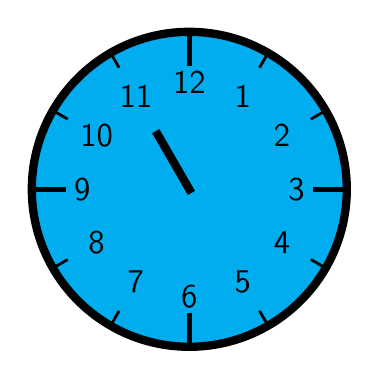
\begin{tikzpicture}[line cap=rect,line width=3pt]
\filldraw [fill=cyan] (0,0) circle [radius=2cm];
\foreach \angle [count=\xi] in {60,30,...,-270}
{
  \draw[line width=1pt] (\angle:1.8cm) -- (\angle:2cm);
  \node[font=\large] at (\angle:1.36cm) {\textsf{\xi}};
}
\foreach \angle in {0,90,180,270}
  \draw[line width=2pt] (\angle:1.6cm) -- (\angle:2cm);
\draw (0,0) -- (120:0.8cm);
\end{tikzpicture}
\]

Suppose that our clock has just an hour hand for now. Then we may collect all
the way things can be for the clock into a set of hours:
$$\Set{Hour} := \{1, 2, 3, 4, 5, 6, 7, 8, 9, 10, 11, 12\}.$$
This set $\Set{Hour}$ is the set of \emph{states} of our clock system.

If we know what hour it is, we also know what hour is coming next. So, this system has the following dynamics:
%
% :CUSTOM-ID: problem-with-drawing-mapsto-nicely
%
\begin{align}\label{eqn.tick}
  \fun{tick} : \Set{Hour} &\to \Set{Hour} \\\nonumber
                t &\mapsto \begin{cases} t + 1 &\mbox{if $t < 12$}\\ 1 &\mbox{if $t = 12$}  \end{cases}
\end{align}

Here's a sample of the dynamics of the clock. Say we started at the 10 o'clock state:
$$10 \xmapsto{\fun{tick}} 11 \xmapsto{\fun{tick}} 12 \xmapsto{\fun{tick}} 1 \To{\fun{tick}} 2
\xmapsto{\fun{tick}} \cdots$$

Ok, it's not the most dynamic of systems, but we have to start somewhere. If we want to
refer to the whole system at once, we can box it up and draw it like this:

\begin{equation}\label{eqn.clock_system_box}
\begin{tikzpicture}[oriented WD, every fit/.style={inner xsep=\bbx, inner ysep=\bby}, bbx = 1cm, bby =.5cm, bb min width=1cm, bb port length=4pt, bb port sep=1, baseline=(X.center)]
	\node[bb={0}{1}, fill=blue!10] (X) {$\Sys{Clock}$};
	\draw[label] 
		node [right=2pt of X_out1] {$\Set{Hour}$}
		;
\end{tikzpicture}
\end{equation}
We imagine that the clock is going about its business inside the box, and
that is shows the hour it is currently displaying on the outgoing wire. This outgoing wire constitutes the clock's exposed variable, but we'll explain that more later.

One issue with our clock is that it doesn't tell us whether it is morning or
evening. Being morning or evening and going back and forth between them is another way that things might be and change, and hence we
can see it as its own two-state dynamical system with states
$$\Set{a.m./p.m.} = \{\const{a.m.}, \const{p.m.}\}.$$

However, rather than have this be an independent system, we want to consider it as a little addition to
our clock system, one that reads $\const{a.m.}$ or $\const{p.m.}$:
\begin{equation}\label{eqn.whole_clock}
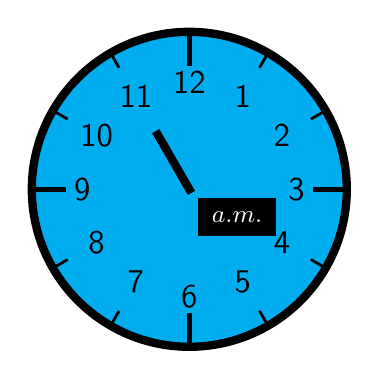
\begin{tikzpicture}[line cap=rect,line width=3pt, baseline=(bl)]
\coordinate (bl) at (0,0);
\filldraw [fill=cyan] (0,0) circle [radius=2cm];
\foreach \angle [count=\xi] in {60,30,...,-270}
{
  \draw[line width=1pt] (\angle:1.8cm) -- (\angle:2cm);
  \node[font=\large] at (\angle:1.36cm) {\textsf{\xi}};
}
\foreach \angle in {0,90,180,270}
  \draw[line width=2pt] (\angle:1.6cm) -- (\angle:2cm);
\draw (0,0) -- (120:0.8cm);
\node[draw, fill] at (330:.7cm) {\small${ \color{white}\const{a.m.} }$};
\end{tikzpicture}
\end{equation}
To connect the meridian to the clock means that the way the meridian changes should be based on the hour:
\begin{align}\label{eqn.next}
  \fun{next} : \Set{a.m./p.m.} \times \Set{Hour} &\to \Set{a.m./p.m.} \\\nonumber
               (\const{a.m.}, t) &\mapsto \begin{cases} \const{p.m.} &\mbox{if $t = 11$}\\ \const{a.m.} &\mbox{otherwise}  \end{cases} \\\nonumber
               (\const{p.m.}, t) &\mapsto \begin{cases} \const{a.m.} &\mbox{if $t = 11$}\\ \const{p.m.} &\mbox{otherwise}  \end{cases}
\end{align}
If it is $\const{a.m.}$ and the clock reads 8, then it will still be
$\const{a.m.}$ at the next tick; but if it is $\const{a.m.}$ and the clock reads 11, then the next tick will switch the meridian to $\const{p.m.}$.

Again, the thing to note about the dynamics of the $\const{a.m.}/\const{p.m.}$ system
is that they depend on what hour it is. The hour is imported as a \emph{parameter} for the
dynamics of the meridian system. We can draw the meridian system as a box like this:
\begin{equation}\label{eqn.am_pm_system_box}
\begin{tikzpicture}[oriented WD, every fit/.style={inner xsep=\bbx, inner ysep=\bby}, bbx = 1cm, bby =.5cm, bb min width=1cm, bb port length=4pt, bb port sep=1, baseline=(X.center)]
	\node[bb={1}{1}, fill=blue!10] (X) {$\Sys{Meridian}$};
	\draw[label] 
		node [left=2pt of X_in1] {$\Set{Hour}$}
		node [right=2pt of X_out1] {$\Set{a.m./p.m.}$}
		;
\end{tikzpicture}
\end{equation}
We have the $\Set{a.m./p.m.}$ wire coming out, which carries the information of
whether it is $\const{a.m.}$ or $\const{p.m.}$, just like the clock. But we also
have a wire coming in, which carries the hour that we need as a parameter for
our dynamics.


We can now express our whole clock \eqref{eqn.whole_clock} by wiring together
our bare clock \eqref{eqn.clock_system_box} and the $\const{a.m.}/\const{p.m.}$ system:

\begin{equation}\label{eqn.whole_clock_system_box}
\begin{tikzpicture}[oriented WD, every fit/.style={inner xsep=\bbx, inner ysep=\bby}, bbx = .3cm, bby =.3cm, bb min width=.5cm, bb port length=2pt, bb port sep=1, baseline=(Y.center)]
	\node[bb={1}{1}, fill=blue!10] (X1) {$\Sys{Meridian}$};
  	\node[bb={0}{1}, fill=blue!10, below=2 of X1] (X2) {$\Sys{Clock}$};
	\node[bb={0}{2}, fit={($(X1.north west)+(-2,1)$) ($(X1.north east)+(2,1)$) ($(X2.south)+(0,-3)$)}] (Y) {};
  \node[above=0pt of Y.south] (Label) {$\Sys{ClockWithDisplay}$};
	\draw (X1_out1) to (Y_out1);
  \draw let \p1=(X1.south west), \p2=(X2.north east), \n1=\bbportlen, \n2=\bby in
    (X2_out1) to[in=0] (\x2 + \n1, \y2 + \n2) -- (\x1 - \n1, \y2 + \n2) to[out=180] (X1_in1);
  \draw (X2_out1) to (Y_out2);
	\draw[label] 
		node [right=2pt of Y_out1] {$\Set{a.m./p.m.}$}
		node [right=2pt of Y_out2] {$\Set{Hour}$}
		;
\end{tikzpicture}
\end{equation}

The resulting system has states
$$\Set{HoursWithDisplay} := \Set{Hour} \times \Set{a.m./p.m.}$$
each of which is a pair, e.g.\ $(11, \const{a.m.})$, consisting of an hour and a meridian reading.
They update in a combined way, by using the hour shown on the clock face as the
parameter we need for the $\Sys{Meridian}$ system; this is expressed by having a wire from the output of $\Sys{Clock}$ to the input of $\Sys{Meridian}$. In full, the
dynamics looks like this:
\begin{align*}
  \fun{tick'} :\Set{HoursWithDisplay} &\to \Set{HoursWithDisplay} \\
  (t, m) &\mapsto (\fun{tick}(t), \fun{next}(t, m))
\end{align*}
where $\fun{tick}$ and $\fun{next}$ are as in \eqref{eqn.tick} and \eqref{eqn.next}.

\begin{exercise}
  Expand the definition of the combined system out in full, and check that it
  really does behave like the clock with $\const{a.m.}/\const{p.m.}$ display should.
\end{exercise}

Now that we have a working clock, we can use it for systems that need to know
the time. For example, consider a diner that opens at $7 \const{a.m.}$ and
closes at $10 \const{p.m.}$. The states of this diner are
$$\Set{DinerState} = \{\const{open}, \const{closed}\}.$$
The diner's dynamics are then
\begin{align*}
  \fun{dinerDynamics} : \Set{DinerState} \times \Set{HoursWithDisplay} &\to \Set{DinerState} \\
  (\const{open}, (10, \const{p.m.})) &\mapsto \const{closed} \\
  (\const{closed}, (7, \const{a.m.})) &\mapsto \const{open} \\
  (s, (t, m)) &\mapsto s \quad\mbox{otherwise.} 
\end{align*}

Again, we can represent the diner by this box:
\begin{equation}\label{eqn.diner_system_box}
\begin{tikzpicture}[oriented WD, every fit/.style={inner xsep=\bbx, inner ysep=\bby}, bbx = 1cm, bby =.5cm, bb min width=1cm, bb port length=4pt, bb port sep=1, baseline=(X.center)]
	\node[bb={2}{1}, fill=blue!10] (X) {$\Sys{Diner}$};
	\draw[label] 
		node [left=2pt of X_in1] {$\Set{a.m./p.m.}$}
		node [left=2pt of X_in2] {$\Set{Hour}$}
		node [right=2pt of X_out1] {$\Set{DinerState}$}
		;
\end{tikzpicture}
\end{equation}
This time, we have two wires coming in, corresponding to the two parameters we
need for the diner system: the hour and the
meridien. 

Assuming that the diner has a clock on its wall which it uses to decide whether
to open or close, the full diner system would be given by wiring the clock with display into
those input wires:
\begin{equation}\label{eqn.diner_system_box}
\begin{tikzpicture}[oriented WD, every fit/.style={inner xsep=\bbx, inner ysep=\bby}, bbx = 1cm, bby =.5cm, bb min width=1cm, bb port length=4pt, bb port sep=1, baseline=(Outer.center)]
  \node[bb={0}{2}, fill=blue!10](Clock) {$\Sys{ClockWithDisplay}$};
  \node[bb={2}{1}, fill=blue!10, right=of Clock] (Diner) {$\Sys{Diner}$};
  
  \node[bb={0}{1}, fit={(Clock) (Diner)}] (Outer) {};

  \draw (Clock_out1) to (Diner_in1);
  \draw (Clock_out2) to (Diner_in2);
  \draw (Diner_out1) to (Outer_out1);

  \draw[label] node [right=2pt of Outer_out1] {$\Set{DinerState}$};
\end{tikzpicture}
\end{equation}
If we want to, we can peak into the clock with display and see that it is itself
made out of a clock wired to a display:
\begin{equation}\label{eqn.diner_system_box}
\begin{tikzpicture}[oriented WD, every fit/.style={inner xsep=\bbx, inner ysep=\bby}, bbx = 1cm, bby =.3cm, bb min width=1cm, bb port length=4pt, bb port sep=1, baseline=(Outer.center)]
	\node[bb={1}{1}, fill=blue!10] (X1) {$\Sys{Meridian}$};
  	\node[bb={0}{1}, fill=blue!10, below=2 of X1] (X2) {$\Sys{Clock}$};
	\node[dashed, bb={0}{2}, fit={($(X1.north west)+(0,1)$) ($(X1.north east)+(0,1)$) ($(X2.south)+(0,-3)$)}] (Clock) {};
  \node[above=0pt of Clock.south] (Label) {$\Sys{ClockWithDisplay}$};
	\draw (X1_out1) to (Clock_out1);
  \draw let \p1=(X1.south west), \p2=(X2.north east), \n1=\bbportlen, \n2=\bby in
    (X2_out1) to[in=0] (\x2 + \n1, \y2 + \n2) -- (\x1 - \n1, \y2 + \n2) to[out=180] (X1_in1);
  \draw (X2_out1) to (Clock_out2);
  \node[bb={2}{1}, fill=blue!10, right=of Clock] (Diner) {$\Sys{Diner}$};
  
  \node[bb={0}{1}, fit={(Clock) (Diner)}] (Outer) {};

  \draw (Clock_out1) to (Diner_in1);
  \draw (Clock_out2) to (Diner_in2);
  \draw (Diner_out1) to (Outer_out1);

  \draw[label] node [right=2pt of Outer_out1] {$\Set{DinerState}$};
\end{tikzpicture}
\end{equation}

These examples are simple, but it doesn't take much more to get to some truly
amazing phenomena. Consider this system: we have an infinite tape with a
read-head at some integer position. On this infinite tape, we will write the symbols
$a$, $b$, $c$, or $d$, or we will leave it blank: $\_$. Together, the state
of the tape and the position of the read-head have states pairs $(\fun{T}, n)$ consisting of a
function $\fun{T} : \zz \to \{a, b,c,d,\_\}$, telling us what symbol $\fun{T}(i)$ is found at
position $i$ of the tape, and a position $n$ of the read-head:
\begin{align*}
  \Set{Symbol} &= \{a, b,c,d,\_\}\\
  \Set{Tape} &= \Set{Symbol}^{\zz}\\
  \Set{Head} &= \zz
\end{align*}
The parameters that this system needs in order to change are a move-command and a
write-command. The move-command will be either move left or move right, encoded as $-1$ or $1$ respectively, and the write command will be one of the
symbols that can be written on the tape:
\[
  \Set{Move}=\{-1,1\}\qqand
  \Set{Write} = \{a,b,c,d,\_\}.
\]

The way this system changes is by writing the write command to the tape at the current
position, and then moving according to the move command. As a function, this is:
\begin{align*}
  \fun{execute} : \Set{Head} \times \Set{Tape} \times \Set{Move} \times \Set{Write} &\to \Set{Head} \times \Set{Tape}\\
  (n, i\mapsto \fun{T}(i), d, s) &\mapsto \left( n + d, i \mapsto \begin{cases} \fun{T}(i) &\mbox{if $i \neq n$} \\ s &\mbox{if $i = n$} \end{cases} \right).
\end{align*}

We can imagine that the system exposes the tape and the symbol under its read head. We can box this system up and draw it like so:
\begin{equation}\label{eqn.turing_box}
\begin{tikzpicture}[oriented WD, every fit/.style={inner xsep=\bbx, inner ysep=\bby}, bbx = 1cm, bby =.5cm, bb min width=1cm, bb port length=4pt, bb port sep=1, baseline=(Tape.center)]
\node[bb={2}{2}, fill=blue!10] (Tape) {$\Sys{Tape Machine}$};
\draw[label]
  node[left=2pt of Tape_in1] {$\Set{Move}$}
  node[left=2pt of Tape_in2] {$\Set{Write}$}
  node[right=2pt of Tape_out1] {$\Set{Tape}$}
  node[right=2pt of Tape_out2] {$\Set{Symbol}$}
;
\end{tikzpicture}
\end{equation}

Now, we need one more simple ingredient to get our system going; a mysterious system of the
form:
\begin{equation}\label{eqn.turing_box2}
\begin{tikzpicture}[oriented WD, every fit/.style={inner xsep=\bbx, inner ysep=\bby}, bbx = 1cm, bby =.5cm, bb min width=1cm, bb port length=4pt, bb port sep=1, baseline=(Box.center)]
\node[bb={1}{2}, fill=blue!10] (Box) {$\Sys{Mystery Box}$};
\draw[label]
  node[right=2pt of Box_out1] {$\Set{Move}$}
  node[right=2pt of Box_out2] {$\Set{Write}$}
  node[left=2pt of Box_in1] {$\Set{Symbol}$}
;
\end{tikzpicture}
\end{equation}

We can see that our mystery box will take in a symbol and put out a move command
and a write command. The way our mystery box behaves is rather mysterious. It has six states $S\cong\6$, and its update rule is given by the following table,
where the entry in the row $i$ and the column $s$ is written $(m,w):s'$ to express the
move command $m$, the write command $w$, and the next state $s'$ that our
mysterious system transitions to when input the symbol $i$ in state $s$:
\begin{equation}\label{eqn.turing_machine}
  \begin{tabular}{|c|c|c|c|c|c|c|}
    \hline
     & 1 & 2 & 3 & 4 & 5 & 6 \\\hline
    a & (-1, b):1 & (1, a):1 & (-1, b):3  & (1, b):2 & (-1, b):6 & (-1, b):4 \\\hline     
   b & (-1, a):1 & (1, a):2 & (-1, b):5  & (1, a):4 & (1, a):6 & (1, a): 5 \\\hline     
   c & (1, d):2 & (1, d):2 & (-1, c):5 & (1,d):4 & (1, c):5 & (1, a):1 \\\hline     
   d & (-1, c):1 & (1, a):5 & (-1, c):3 & (1,d):5 & (-1, b):3 & end \\\hline     
  \end{tabular}
\end{equation}
Mysterious indeed. But when we wire the two together, magic happens!

\begin{equation}\label{eqn.full_turing_machine}
\begin{tikzpicture}[oriented WD, every fit/.style={inner xsep=\bbx, inner ysep=\bby}, bbx = 1cm, bby =.5cm, bb min width=1cm, bb port length=2pt, bb port sep=1, baseline=(Outer.center)]
  \node[bb={1}{2}, fill=blue!10](Box) {$\Sys{Mystery Box}$};
  \node[bb={2}{2}, fill=blue!10, right=of Box] (Tape) {$\Sys{Tape Machine}$};
  
  \node[bb={0}{0}, fit={($(Tape.south east) + (0, -2)$) ($(Box.north west) + (0, 1)$)}] (Outer) {};
  \node[above=0pt of Outer.south] (Label) {$\Sys{Universal Turing Machine}$};

  \draw (Box_out1) to (Tape_in1);
  \draw (Box_out2) to (Tape_in2);

  \draw (Tape_out1) to (Outer.east|-Tape_out1);
  \draw (Tape_out2) to (Outer.east|-Tape_out2);

  \draw let \p1=(Tape.south east), \p2=(Box.south west), \n1=\bbportlen, \n2=\bby in
    (Tape_out2) to[in=0] (\x1 + \n1, \y1 - \n2 - 1) -- (\x2 - \n1, \y2 - \n2 - 1) to[out=180] (Box_in1);
\end{tikzpicture}
\end{equation}
This is a universal Turing machine, i.e.\ when we encode everything into this strange alphabet, it is capable of arbitrarily complex calculation! 
\slogan{Even simple systems can
have very interesting behavior when plugged in to the right environment.}

%%
%% :CUSTOM_ID:cite-this.turing_machine
%% 
That's a lot of informal definitions, we are ready for something precise:
\begin{definition}\label{def.deterministic_system}
  A \emph{deterministic system} $\Sys{S}$, also written as 
  $$\lens{\update{S}}{\expose{S}} : \lens{\State{S}}{\State{S}} \leftrightarrows \lens{\In{S}}{\Out{S}},$$ 
  consists of:
  \begin{itemize}
    \item a set $\State{S}$ of \emph{states};
    \item a set $\Out{S}$ of \emph{values for exposed variables}, or \emph{outputs}
      for short;
    \item a set $\In{S}$ of \emph{parameter values}, or \emph{inputs} for short;
    \item a function $\expose{S} : \State{S} \to \Out{S}$, the \emph{exposed variable of state} or
      \emph{expose} function, which takes a state to the output it yields; and
    \item a function $\update{S} : \State{S} \times \In{S} \to \State{S}$, the \emph{dynamics} or
      \emph{update} function which takes a state and a parameter and gives the
      next state.
  \end{itemize}
  We refer to the pair $\lens{\In{S}}{\Out{S}}$ of exposed variable and parameter values as
  the \emph{interface} of the system.

We can interpret this definition in any cartesian category $\cat{C}$; here, we
have have used the category $\Cat{Set}$ of sets.
\end{definition}

\begin{remark}
  Deterministic systems are also known as \emph{Moore machines} in the
  literature. If the output set is taken to be $\{\const{true},
  \const{false}\}$, then they are known as \emph{deterministic automata}.

  Often, these definitions also include a \emph{start state} $s_0 \in \State{S}$
  as part of the data. We don't do this.
\end{remark}

\begin{example}\label{ex.clock_system}
  The $\Sys{Clock}$ system can be seen as a deterministic system with:
  $$\lens{\fun{tick}}{\id} : \lens{\Set{Hour}}{\Set{Hour}} \fromto \lens{\{\ast\}}{\Set{Hour}}.$$
  In other words, it consists of
  \begin{itemize}
  \item State set $\State{Clock} = \Set{Hour} =\{1,2,\ldots,12\}$.
  \item Output set $\Out{Clock} = \Set{Hour}$.
  \item Input set $\In{Clock} = \{\ast\}$, a one element set.
  \item Readout function $\expose{Clock} = \id_{\Set{Hour}}$.
  \item update function $\update{Clock} : \Set{hours} \times \{\ast\} \to \Set{Hour}$
    defined by $\update{Clock}(t, \ast) = \fun{tick}(t)$.
  \end{itemize}
\end{example}

\begin{example}\label{ex.moore_machine}
  The term \emph{Moore machine} is often used for the mathematical notion of
  deterministic system we've just presented, but it is also used for actual,
  real-life circuits which are designed on that principle.

  For example, suppose that a wire carries the signals $\Set{Wire} =
  \{\const{high}, \const{low}\}$. We can see a deterministic system $\Sys{M}$
  with input $\In{M} = \Set{Wire}^n$ and $\Out{M} = \Set{Wire}^k$ as a circuit
  with $n$ incoming wires and $k$ outgoing wires.\footnote{Of course, the notion
  of ``incoming'' and ``outgoing'' wires are ways we think about the circuit in
  design terms. Circuits aren't actually directed in this way. We'll think about
undirected notions of system in \cref{chapter.2}.} The state then describes the
state of all the internal wires (and capacitors, etc.) in the circuit. We would wire up these systems by literally wiring them together. 

\jaz{I would like to add an example of an implementation of a Moore machine into
  a circuit.}
%%
%%  :CUSTOM-ID:moore-machine-example
%%
\end{example}

Note that when we say that a system doesn't have any parameters, as in \cref{ex.clock_system}, we don't take the
parameter set to be empty but instead take it to have a single dummy value $\{*\}$, the one-element ``hum of existence''. In other words, having ``no parameters'' really means that the parameters are unchanging, or that there is no way to change the value of the parameters.

Also, we are just exposing the whole state with the system in \cref{ex.clock_system}. There is nothing preventing our systems
from exposing their whole state, but often some aspects of the state are private, i.e.\ not exposed for use by other systems. 

\begin{exercise}\label{exc.clock_meridian_diner}
  Write out the clock and meridian systems from \eqref{eqn.tick} and \eqref{eqn.next} in terms of
  \cref{def.deterministic_system}. Really, this amounts to noticing which sets
  are the sets of states, which are the sets of inputs, and what (implicitly)
  are the sets of outputs.
\end{exercise}

\begin{example}[SIR model]\label{ex.SIR_model_discrete}
  The set of states for a deterministic system doesn't need to be finite. The $\Sys{SIR}$ model
  is an epimediological model used to study how a disease spreads through a
  population. ``SIR'' stands for ``susceptible'', ``infected'', and, rather
  ominously, ``removed''. This model is usually presented as a system of
  differential equations --- what we will call a differential system --- and we will see it in that form in \cref{ex.SIR_model_diff}.
  But we can see a discrete approximation to this continuous model as a
  deterministic system.

  A state of the $\Sys{SIR}$ model is a choice of how many people are susceptible, how
  many are infected, and how many are removed. That is,
  $$\State{SIR} = \left\{\begin{bmatrix} s \\ i \\ r \end{bmatrix}\; \middle|\; s,\, i,\, r\in \rr\right\} \cong \rr^3.$$
  is a 3-place vector of real numbers. We will again expose the whole state, so
  $\Out{SIR} = \State{SIR}$ and $\expose{SIR} = \id$.

  The idea behind the $\Sys{SIR}$ model is that if a susceptible person comes in
  contact with an infected person, then they have a chance of becoming infected
  too. And, eventually, infected persons will be removed from the model, either
  by recovering (a gentler way to read the ``R'') or by dying. So we need two
  parameters: the rate $a$ of infection and the rate $b$ of removal:
  $$\In{SIR} = \left\{\begin{bmatrix} a \\ b \end{bmatrix}\, \middle|\, a,\, b \in \rr\right\} = \rr^2.$$

  Now, we can show how a population will develop according to this model by
  defining the update function:
  \begin{align}\label{eqn.SIR_model_discrete}
    \update{SIR} : \State{SIR} \times \In{SIR} &\to \State{SIR}\\
    \left( \begin{bmatrix} s\\ i\\ r\\ \end{bmatrix},\, \begin{bmatrix}a \\ b \end{bmatrix} \right) &\mapsto \begin{bmatrix}s - a s i \\ i + a s i - b  i \\ r + b i \end{bmatrix}
  \end{align}

\end{example}

\begin{example}\label{ex.transition_diagram_discrete}
  If a deterministic system has a small finite set of states, then we can draw it
entirely as a \emph{transition diagram}:

\[
\begin{tikzpicture}
	\node[draw] {
  \begin{tikzcd}[column sep=small]
  	\LMOO{1}{a}\ar[rr, dgreen, thick, bend left]\ar[loop left, thick, orange]&&
  	\LMOO{2}{b}\ar[ll, thick, orange, bend left]\ar[dl, bend left, thick, dgreen]\\&
  	\LMOO{3}{b} \ar[ul, thick, orange, bend left] \ar[loop left, thick, dgreen]
  \end{tikzcd}
  };
\end{tikzpicture}
\]
Note that every node has an orange and a green arrow emanating from it, but that there are no rules on how many arrows point to it.

This diagram describes the following system $\Sys{S}$:
  $$\lens{\update{S}}{\expose{S}} : \lens{\{1, 2, 3\}}{\{1, 2, 3\}} \leftrightarrows \lens{\{{\color{dgreen} \const{green},\, {\color{orange} \const{orange}}}\}}{\{a, b\}}.$$ 
That is, we have
\begin{itemize}
\item $\State{S} = \{1, 2, 3\}$.
\item $\In{S} = \{{\color{dgreen} \const{green},\, {\color{orange} \const{orange}}}\}$,
\item $\Out{S} = \{a, b\}$,
\item \[\begin{aligned}
        \expose{S} : \State{S} &\to \Out{S} \\
        1 &\mapsto a \\
        2 &\mapsto b \\
        3 &\mapsto b \\~\\~\\~\\
      \end{aligned} \quad\quad\quad\quad
 \begin{aligned}
        \update{S} : \State{S} \times \In{S} &\to \In{S} \\
        (1, {\color{dgreen} \const{green}}) &\mapsto 2 \\
        (1, {\color{orange} \const{orange}}) &\mapsto 1 \\
        (2, {\color{dgreen} \const{green}}) &\mapsto 3 \\
        (2, {\color{orange} \const{orange}}) &\mapsto 1 \\
        (3, {\color{dgreen} \const{green}}) &\mapsto 3 \\
        (3, {\color{orange} \const{orange}}) &\mapsto 1
      \end{aligned}
      \]
\end{itemize}

To draw a transition diagram of a system $\Sys{S}$, we draw each state $s \in
\State{S}$ as a bubble filled with the label $\expose{S}(s)$, and for each
parameter $i \in \In{S}$ we draw an arrow from $s$ to $\update{S}(s, i)$. For a
diagram like this to be a transition diagram, every node must have an edge
leaving it for each parameter.
\end{example}

\begin{exercise}
  Draw the $\Sys{Clock}$ system (\cref{ex.clock_system}) as a transition diagram.
\end{exercise}

\begin{example}[Deterministic Finite Automata]\label{ex.dfa}
  A \emph{deterministic finite automaton} (DFA) is a simple model of computation.
  Given our definition of deterministic system, DFAs are easy enough to define:
  they are just the deterministic systems with finitely many states whose output values are either
  $\const{true}$ or $\const{false}$. 

  This means that the exposed variable of state $\expose{S} : \State{S} \to
  \{\const{true},\, \const{false}\}$ is a boolean valued function. We say a
  state $s$ is an \emph{accept state} if $\expose{S}(s) = \const{true}$, and a
  \emph{reject state} if $\expose{S}(s) = \const{false}$.

  The idea is that a DFA is a question answering machine. Given a starting state
  $s_0$ and a sequence of input values $i_1, \ldots, i_n$, we get a sequence of
  states by $s_{t+1}:= \update{S}(s_t, i_t)$. The answer to the question is
  ``yes'' if $s_n$ is an accept state, and ``no'' if $s_n$ is a reject state.

\end{example}

There is an important special case of deterministic systems which appear very
commonly in the literature: the \emph{closed} systems. These are the systems
which have no parameters, and which expose no variables. They are closed off
from their environment, and can't be wired into any other systems.

As mentioned after \cref{ex.clock_system}, when we say ``no'' in this way --- no parameters, no variables --- we should be
careful with what we mean exactly. We mean that there is no \emph{variation} in
the parameters or variables, that they are trivial. That is, we make the
following definition.
\begin{definition}
  A deterministic system $\Sys{S}$ is \emph{closed} if both $\In{S}$ and
  $\Out{S}$ have only one element
  \[\In{S}\cong\{*\}\cong\Out{S}.\]
\end{definition}

\begin{exercise}
Show that to give a closed system
\[\lens{\update{S}}{\expose{S}}\colon\lens{\State{S}}{\State{S}}\fromto\lens{\{*\}}{\{*\}},\]
one just needs to choose a set $\State{S}$ and an update function $\update{S} :  \State{S} \to \State{S}$.
\end{exercise}

Given that we are mostly interested in how systems wire together, it may seem
strange to draw attention to the closed systems that \emph{can't} be wired into
anything else. But we will often end up with a closed system as the result of
wiring together some systems.

For example, suppose we have an $\Sys{Agent}$ acting within a
$\Sys{Environment}$. The agent will take an action, and the evironment will
respond to that action. Depending on the action taken and response given, the
agent and the environment will update their states. We can model this by the
following wiring diagram:
\[
\begin{tikzpicture}[oriented WD, every fit/.style={inner xsep=\bbx, inner ysep=\bby}, bbx = 1cm, bby =.5cm, bb min width=1cm, bb port length=2pt, bb port sep=1, baseline=(Outer.center)]
  \node[bb={1}{1}, fill=blue!10](Box) {$\Sys{Agent}$};
  \node[bb={1}{1}, fill=blue!10, right=of Box] (Tape) {$\Sys{Environment}$};
  
  \node[bb={0}{0}, fit={($(Tape.south east) + (0, -2)$) ($(Box.north west) + (0, 1)$)}] (Outer) {};
  \node[above=0pt of Outer.south] (Label) {$\Sys{Closed\ Agent/Environment\ Model}$};

  \draw (Box_out1) to (Tape_in1);


  \draw let \p1=(Tape.south east), \p2=(Box.south west), \n1=\bbportlen, \n2=\bby in
    (Tape_out1) to[in=0] (\x1 + \n1, \y1 - \n2 - 1) -- (\x2 - \n1, \y2 - \n2 - 1) to[out=180] (Box_in1);
\end{tikzpicture}
\]

To have this be a closed model is to think --- or pretend --- that the our model
of the $\Sys{Agent}$ and the $\Sys{Environment}$ includes all possible external
parameters, that it is well isolated from its own environment.

\begin{exercise}
What would happen to a system $\Sys{S}$ if its set of parameters or output values were actually empty sets? Let's find out.
\begin{enumerate}
	\item Suppose $\In{S}=\varnothing$. Explain the content of a deterministic system \[\lens{\update{S}}{\expose{S}}\colon\lens{\State{S}}{\State{S}}\fromto\lens{\varnothing}{\{*\}}.\]
	\item Suppose $\Out{S}=\varnothing$. Explain the content of a deterministic system \[\lens{\update{S}}{\expose{S}}\colon\lens{\State{S}}{\State{S}}\fromto\lens{\{*\}}{\varnothing}.
	\qedhere
\]	
\end{enumerate}
\end{exercise}



\subsection{Differential systems}

\begin{quote}
  \emph{La nature ne fait jamais des sauts} - Liebniz
\end{quote}

A quirk of modeling dynamical systems as determinstic systems is that
determinstic systems lurch from one state to the next. In life, there are no
next moments. Time, at least at human scales and to a first approximation, flows
continuously.

Instead of modelling the ``next'' state a system will be in, we can model
\emph{how the system is tending to change}, in the moment. In order to do this,
we need to make concession in the way we model the states of our system: we must
assume they form a continuum themselves.

For example, suppose we are studying a population of $\Sys{Rabbits}$. We can
measure the rate at which rabbits are born, and the rate they die. Then the
population changes according to these rates. We can express this dependency of
the change in population on certain rates with a differential equation:
\[
\frac{dr}{dt} = \const{b}_{\Sys{Rabbits}} \cdot r - \const{d}_{\Sys{Rabbits}}
\cdot r
\]
where $r \in \rr$ is the population of rabbits (considered as a real number for
convenience), and the rates $\const{b}_{\Sys{Rabbits}}$ and
$\const{d}_{\Sys{Rabbits}}$. The state of our system of $\Sys{Rabbits}$ is the current population of rabbits,
so $\State{Rabbits} = \rr$, while we take the birth and death rates as
parameters, so that $\In{Rabbits} = \rr \times \rr$. Accordingly, 
we can box the rabbit system up like so:
\begin{equation}\label{eqn.rabbit_box}
\begin{tikzpicture}[oriented WD, every fit/.style={inner xsep=\bbx, inner ysep=\bby}, bbx = 1cm, bby =.5cm, bb min width=1cm, bb port length=4pt, bb port sep=1, baseline=(Tape.center)]
\node[bb={2}{1}, fill=blue!10] (Tape) {$\Sys{Rabbits}$};
\draw[label]
  node[left=2pt of Tape_in1] {$\rr$}
  node[left=2pt of Tape_in2] {$\rr$}
  node[right=2pt of Tape_out1] {$\rr$}
;
\end{tikzpicture}
\end{equation}

Now, rabbits are prey; they are eaten by other animals. That means that the rate
at which rabbits die will depend on how often they are being eaten, and how
often they are being eaten will depend on how many predators there are out there.

Now, the population of any predator will also change according to a birth rate
and death rate. Suppose we have a similarly defined system of $\Sys{Foxes}$
goverened whose population is governed by the differential equation
\[
\frac{df}{dt} = \const{b}_{\Sys{Foxes}} \cdot f - \const{d}_{\Sys{Foxes}}
\cdot f.
\]
We can box up this system like so:
\begin{equation}\label{eqn.foxes_box}
\begin{tikzpicture}[oriented WD, every fit/.style={inner xsep=\bbx, inner ysep=\bby}, bbx = 1cm, bby =.5cm, bb min width=1cm, bb port length=4pt, bb port sep=1, baseline=(Tape.center)]
\node[bb={2}{1}, fill=blue!10] (Tape) {$\Sys{Foxes}$};
\draw[label]
  node[left=2pt of Tape_in1] {$\rr$}
  node[left=2pt of Tape_in2] {$\rr$}
  node[right=2pt of Tape_out1] {$\rr$}
;
\end{tikzpicture}
\end{equation}

Now, we want the death rate of rabbits to depend on the number of foxes. But we
also need the birth rate of the foxes to depend on the number of rabbits; after
all, if a fox has nothing to eat, it has no time for hanky-panky. So we will add the following
system of equations to the mix:
\[
\begin{cases} \const{d}_{\Sys{rabbits}} = c_1 f \\ \const{b}_{\Sys{Foxes}} =
  c_2 r \end{cases}
\]
Making these
substitutions, we get the following system of differential equations:
\[
  \begin{cases}
    
\frac{dr}{dt} =  \const{b}_{\Sys{Rabbits}}
\cdot r - c_1 f r \\
\frac{df}{dt} = c_2 r f - \const{d}_{\Sys{Foxes}}
\cdot f
  \end{cases}
\]

We are setting the parameters of the systems of $\Sys{Rabbits}$ and
$\Sys{Foxes}$ according to the states of the other system. That is, we are
wiring up the systems of $\Sys{Rabbits}$ and $\Sys{Foxes}$:
\begin{equation}
\begin{tikzpicture}[oriented WD, bb min width =.5cm, bbx=.5cm, bb port sep =1,bb port length=0, bby=.15cm, baseline=(Z.center)]
  \node[bb={4}{1}, fill=blue!10] (rabbit) {$\Sys{Rabbits}$};
  \node[bb={4}{1}, fill=blue!10, below = 8 of rabbit] (fox) {$\Sys{Foxes}$};

  \node[draw=dgreen, circle, inner sep = 0] (c2) at ($(fox_out1) + (2, 2)$){$c_2$};
  \node[draw=dgreen, circle, inner sep = 0, ] (c1) at ($(rabbit_out1-|fox_out1) + (2, -2)$) {$c_1$};

  \node[bb={2}{2}, fit = {($(rabbit.north east) + (5,2)$ ) ($(rabbit.north west) + (-2,0)$) ( $(fox.south east) + (5, -2)$ ) ($(fox.south west) + (-2, 0)$)}] (Z) {};

 \draw (rabbit_out1) to ($(rabbit_out1-|Z_out1) + (0,2)$);
 \draw (rabbit_out1) to[in=170] (c1);
 \draw (rabbit_in1-|Z_in1) to (rabbit_in1);
 \draw (fox_out1) to ($(fox_out1-|Z_out1) + (0,-2)$);
 \draw (fox_out1) to (c2);
 \draw (fox_in4-|Z_in1) to (fox_in4);

 \coordinate[below = 4 of rabbit] (midpoint);
 \draw (c1) to[out=350, in=10, looseness=2] (midpoint);
 \draw (midpoint) to[out=190, in=180, looseness=3] (fox_in1);
 \draw (c2) to[out=10, in=350, looseness=2] (midpoint);
 \draw (midpoint) to[out=170, in=180, looseness=3] (rabbit_in4);
\end{tikzpicture}
\end{equation}





%% writehere
%-------- Section --------%
\section{Wiring together systems with lenses}\label{sec.wiring_discrete_systems}

In the last section, we saw the formal definition of deterministic systems and a
few examples of them. In this section, we'll see how to wire systems together---as we did in \cref{sec.chap1_intro} for the clock and the universal Turing machine---to
make more complex systems. We will do this using an interesting notion coming
from the world of function programming: a \emph{lens}.

%---- Subsection ----%
\subsection{Lenses and lens composition}\label{sec.lens_discrete}

A lens is a framework for bi-directional information passing.

\begin{definition}\label{def.lens}
  A \emph{lens} $\lens{f^{\sharp}}{f} : \lens{A^-}{A^+} \leftrightarrows
  \lens{B^-}{B^+}$ in a cartesian category $\cat{C}$ consists of:
  \begin{itemize}
  \item A \emph{passforward} map $f : A^+ \to B^+$, and
    \item a \emph{passback} map $f^{\sharp} : A^+ \times B^- \to A^-$.
  \end{itemize}
\end{definition}

The most useful thing about lenses is that they \emph{compose}.
\begin{definition}\label{def.lens_composition}
  Let $\lens{f^{\sharp}}{f} : \lens{A^-}{A^+} \leftrightarrows \lens{B^-}{B^+}$ and
  $\lens{g^{\sharp}}{g} : \lens{B^-}{B^+} \leftrightarrows \lens{C^-}{C^+}$ be lenses in
  a cartesian category $\cat{C}$. We define their composite
  $$\lens{g^{\sharp}}{g} \circ \lens{f^{\sharp}}{f}$$
  to have passforward $g \circ f$ and passback
  $$(a^+, c^-) \mapsto f^{\sharp}\left(a^+, g^{\sharp}(f(a^+), c^-)\right).$$
\end{definition}
Here's a picture so that you can see the information flow for the composite of lenses:%
\footnote{We draw this with a different style---green boxes, etc.---so that the reader will not confuse it with our usual wiring diagrams for systems. These are not dynamic in any way; everything below is just a set.}
\begin{equation}\label{eqn.lens_drawing}
\begin{tikzpicture}[oriented WD, bb small, bb port length=5pt, baseline=(f)]
	\node[bb={1}{1}, rounded corners=5pt, draw=dgreen] (f) {$f$};
	\node[bb={1}{1}, rounded corners=5pt, draw=dgreen, right=1.5 of f] (g) {$g\vphantom{f}$};
	\node[left=0 of f_in1] {$A^+$};
	\node[right=0 of g_out1] {$C^+$};
	\draw (f_out1) to node[above, font=\scriptsize] {$B^+$} (g_in1);
%
	\node[dot, right=6 of g] (dot) {};
	\draw (dot.180) to +(180:5pt) coordinate (dot_in1) node[left] {$A^+$};
	\node[bb={1}{1}, rounded corners=5pt, draw=dgreen] at ($(dot)+(1.5,-1.5)$) (f) {$f$};
	\node[bb={2}{1}, rounded corners=5pt, draw=dgreen, below right=-1 and 2 of f] (g') {$g\shp$};
	\draw (dot) to[out=-60, in=180] (f_in1);
	\draw (f_out1) to node[above=5pt, pos=.6, font=\scriptsize] {$B^+$} (g'_in1);
	\node[bb={2}{1}, rounded corners=5pt, draw=dgreen, above right=-1 and 2 of g'] (f') {$f\shp$};
	\draw (dot) to [out=60, in=180] (f'_in1);
	\draw (g'_out1) to[out=0, in=180] node[below=5pt, font=\scriptsize] {$B^-$} (f'_in2);
	\draw (g'_in2) to (g'_in2-|dot_in1) node[left] {$C^-$};
	\node[right=0 of f'_out1] {$A^-$};
\end{tikzpicture}
\end{equation}

This gives us a category of lenses in any cartesian category $\cat{C}$.

\begin{definition}\label{def.lens_category}
Let $\cat{C}$ be a cartesian category. Then the category $\Cat{Lens}_{\cat{C}}$
has:
\begin{itemize}
\item as objects, the pairs $\lens{A^-}{A^+}$ of objects in $\cat{C}$, which we will
  call \emph{arenas}.
\item as morphisms, the lenses $\lens{f^{\sharp}}{f} : \lens{A^-}{A^+} \leftrightarrows \lens{B^-}{B^+}$.
\item The identity lens is $\lens{\pi_2}{\id} : \lens{A^-}{A^+} \leftrightarrows
  \lens{A^-}{A^+}$, where $\pi_2 : A^+ \times A^- \to A^-$ is the projection.
\end{itemize}
\item Composition is given by lens composition as in \cref{def.lens_composition}.
\end{definition}

\begin{remark}
  The category of lenses is special among categories because it is named for its
  \emph{maps} (which are the lenses), rather than its objects (which are the
  arenas). This is because we will later meet another category, the
  \emph{category of charts} (See \cref{def.category_of_charts}), whose objects are
  the arenas but whose maps are not lenses. Finally, in
  \cref{def.double_category_of_arenas_discrete} we will meet a \emph{double
    category}\footnote{A double category is like a category with two different
    kinds of morphisms and a way for them to commute. See
    \cref{def.double_category} for the precise definition and the accompanying
    discussion.} $\Cat{Arena}_\cat{C}$ which combines these two categories whose objects
  are arenas and which \emph{is} named after its objects. In
  \cref{sec.double_category_of_arenas}, we will explain the name ``arena'' and
  its role in the theory of dynamical systems.
\end{remark}

\begin{exercise}
  \begin{enumerate}
  	\item Draw the composite of two lenses in the style of \eqref{eqn.lens_drawing}.
   	\item Check that $\Cat{Lens}_{\cat{C}}$ is actually a category. That is, check that
    lens composition is associative, and that the identity lens is an identity for it.
  \qedhere
  \end{enumerate}
\end{exercise}

Like any good categorical construction, $\Cat{Lens}_{\cat{C}}$ varies
functorially in its variable cartesian category $\cat{C}$.
\begin{proposition}[Functoriality of $\Cat{Lens}$]\label{prop.lens_functoriality}
  Every cartesian functor $F : \cat{C} \to \cat{D}$ induces a functor
  $\lens{F}{F} : \Cat{Lens}_{\cat{C}} \to \Cat{Lens}_{\cat{D}}$ given by
  $$\lens{F}{F}\lens{f^{\sharp}}{f} = \lens{Ff^{\sharp} \circ \mu\inv}{Ff}$$
  where $\mu = (F\pi_1,\, F\pi_2) : F(X \times Y) \xto{\sim} FX \times FY$ is
  the isomorphism witnessing that $F$ preserves products.
\end{proposition}
\begin{proof}[Proof Sketch.]
  Because lenses are defined just using the cartesian product, and $F$ preserves
  these products, it commutes with everything in sight.
\end{proof}

\begin{exercise}
 \begin{enumerate}
 	\item What does the functor $\lens FF: \Cat{Lens}_{\cat{C}} \to \Cat{Lens}_{\cat{D}}$ do on objects?
	\item Complete the proof of \cref{prop.lens_functoriality}, by showing that $\lens FF$ really is a functor.
	\qedhere
\end{enumerate}
\end{exercise}

%---- Subsection ----%
\subsection{Deterministic systems as lenses}

The reason we are interested in lenses and lens composition is because
deterministic systems are themselves lenses. As written in
\cref{def.deterministic_system}, a system $\Sys{S}$ is a lens
$$\lens{\update{S}}{\expose{S}} : \lens{\State{S}}{\State{S}} \leftrightarrows \lens{\In{S}}{\Out{S}}.$$
In fact, the deterministic systems are precisely the lenses whose input arena is of the form $\lens SS$. This means that we can compose
a system $\Sys{S}$ with a lens $\lens{f^{\sharp}}{f} : \lens{\In{S}}{\Out{S}}
\leftrightarrows \lens{I}{O}$ to get a new dynamical system
$$\lens{f^{\sharp}}{f} \circ \lens{\update{S}}{\expose{S}} :
\lens{\State{S}}{\State{S}} \leftrightarrows \lens{I}{O}$$
with a new interface!

We can use this observation to wire together different systems. We separate this into to phases: first we put two systems in parallel, then we wire them together using a lens. The first phase, combine two systems without having them interact, is achieved through what we call the \emph{parallel product} and denote $\otimes$. Two put two arenas $\lens{A_1}{B_1}$ and $\lens{A_2}{B_2}$ in parallel we just take their product in our cartesian category $\cat{C}$:
\[
\lens{A_1}{B_1}\otimes\lens{A_2}{B_2}\coloneqq\lens{A_1\times A_2}{B_1\times B_2}
\]
In \cref{def.lens_parallel} we define parallel product for morphisms in $\Cat{Lens}$, i.e.\ for general lenses.

\begin{definition}\label{def.lens_parallel}
  For lenses $\lens{f^{\sharp}}{f} : \lens{A_1}{B_2} \leftrightarrows \lens{C_1}{D_1}$ and
  $\lens{g^{\sharp}}{g} : \lens{A_2}{B_2} \leftrightarrows \lens{C_2}{D_2}$, we
  define their \emph{parallel product} $$\lens{f^{\sharp}}{f} \otimes
  \lens{g^{\sharp}}{g} : \lens{A_1 \times A_2}{B_1 \times B_2} \leftrightarrows
  \lens{C_1 \times C_2}{D_1 \times D_2}$$
  to have passforward $f \times g$ and passback
  $$((b_1, b_2), (c_1, c_2)) \mapsto (f^{\sharp}(b_1, c_2), g^{\sharp}(b_2, c_2)).$$
  In terms of morphisms, this is
  $$(B_1 \times B_2) \times (C_1 \times C_2) \xto{\sim} (B_1 \times C_1) \times
  (B_2 \times C_2) \xto{f^{\sharp} \times g^{\sharp}} A_1 \times A_2.$$

  Together with $\lens{\ord{1}}{\ord{1}}$, this gives $\Cat{Lens}_{\cat{C}}$ the
  structure of a monoidal category.
\end{definition}

\begin{remark}
  We will show a slick way to prove that the parallel product does indeed make
  $\Cat{Lens}_{\cat{C}}$ into a monoidal category in \cref{sec.indexed_double_category_of_systems}.
\end{remark}

\begin{exercise}
Show the parallel product of morphisms as in \cref{def.lens_parallel} using the string diagram notation from \eqref{eqn.lens_drawing}.
\end{exercise}


\begin{proposition}\label{prop.lens_functoriality_monoidal}
Let $F : \cat{C} \to \cat{D}$ be a cartesian functor. The induced functor
$\lens{F}{F} : \Cat{Lens}_{\cat{C}} \to \Cat{Lens}_{\cat{D}}$ is strong monoidal
with respect to the parallel product.
\end{proposition}
\begin{proof}
  Since $F$ preserves products, and \jaz{finish}.
\end{proof}

Given two dynamical systems $\Sys{S_1}$ and $\Sys{S_2}$, their parallel product
$\Sys{S_1} \otimes \Sys{S_2}$ is defined explicitly as follows:
\begin{itemize}
\item $\State{S_1 \otimes S_2} := \State{S_1} \times \State{S_2}$.
\item $\Out{S_1 \otimes S_2} := \Out{S_1} \times \Out{S_2}$.
\item $\In{S_1 \otimes S_2} := \In{S_1} \times \In{S_2}$.
\item $\expose{S_1 \otimes S_2}((s_1,\, s_2)) = (\expose{S_1}(s_1),\, \expose{S_2}(s_2))$.
\item $\update{S_1 \otimes S_2}((s_1,\, s_2),\, (i_1,\, i_2)) =
  (\update{S_1}(s_1,\, i_1),\, \update{S_2}(s_2,\, i_2))$.
\end{itemize}

This can be expressed as the following wiring diagram:
\begin{equation}\label{eqn.parallel_product_diagram}
\begin{tikzpicture}[oriented WD, every fit/.style={inner xsep=\bbx, inner ysep=\bby}, bbx = .3cm, bby =.3cm, bb min width=.5cm, bb port length=2pt, bb port sep=1, baseline=(Y.center)]
	\node[bb={1}{1}, fill=blue!10] (X1) {$\Sys{S_1}$};
  \node[bb={1}{1}, fill=blue!10, below=1.5 of X1] (X2) {$\Sys{S_2}$};
	\node[bb={0}{0}, fit={($(X1.north west)+(-2,1)$) ($(X1.north east)+(2,1)$) ($(X2.south)+(0,-2)$)}] (Y) {};
  \node[above=0pt of Y.south] (Label) {$\Sys{S_1 \otimes S_2}$};
  
  \draw[shorten <=-3pt] (X1_in1-|Y.west) to (X1_in1);
  \draw[shorten <=-3pt] (X2_in1-|Y.west) to (X2_in1);

  \draw[shorten >=-3pt] (X1_out1) to (Y.east|-X1_out1);
  \draw[shorten >=-3pt] (X2_out1) to (Y.east|-X2_out1);
\end{tikzpicture}
\end{equation}

If we imagine physically wiring together our boxes, the first thing we would
need to do is collect them together like this; then we can proceed to wire them.
We will do exactly this with our systems: first we will take their parallel
product, and then we compose it with a lens that represents the wiring diagram.

\begin{example}\label{ex.ClockWithDisplay}
 We can describe the $\Sys{ClockWithDisplay}$ system (reproduced below) as a
 composite of lenses.
\begin{equation}\label{eqn.clock_system_box2}
\begin{tikzpicture}[oriented WD, every fit/.style={inner xsep=\bbx, inner ysep=\bby}, bbx = .3cm, bby =.3cm, bb min width=.5cm, bb port length=2pt, bb port sep=1, baseline=(Y.center)]
	\node[bb={1}{1}, fill=blue!10] (X1) {$\Sys{Meridian}$};
  	\node[bb={0}{1}, fill=blue!10, below=2 of X1] (X2) {$\Sys{Clock}$};
	\node[bb={0}{2}, fit={($(X1.north west)+(-2,1)$) ($(X1.north east)+(2,1)$) ($(X2.south)+(0,-3)$)}] (Y) {};
  \node[above=0pt of Y.south] (Label) {$\Sys{ClockWithDisplay}$};
	\draw (X1_out1) to (Y_out1);
  \draw let \p1=(X1.south west), \p2=(X2.north east), \n1=\bbportlen, \n2=\bby in
    (X2_out1) to[in=0] (\x2 + \n1, \y2 + \n2) -- (\x1 - \n1, \y2 + \n2) to[out=180] (X1_in1);
  \draw (X2_out1) to (Y_out2);
	\draw[label] 
		node [right=2pt of Y_out1] {$\Set{a.m./p.m.}$}
		node [right=2pt of Y_out2] {$\Set{Hour}$}
		;
\end{tikzpicture}
\end{equation}

First, we take the parallel product of $\Sys{Meridian}$ and $\Sys{Clock}$ (see \cref{exc.clock_meridian_diner}) to get the system 
$$\Sys{Meridian} \otimes \Sys{Clock} : \lens{\Set{a.m./p.m.} \times \Set{Hour}}{\Set{a.m./p.m.} \times \Set{Hour}} \leftrightarrows \lens{\1\times\Set{Hour}}{\Set{a.m./p.m.} \times \Set{Hour}}.$$

Now, we will express the wiring pattern in \cref{eqn.clock_system_box2} as a lens
$$\lens{w^{\sharp}}{w} : \lens{\1\times\Set{Hour}}{\Set{a.m./p.m.} \times \Set{Hour}} \leftrightarrows \lens{\ord{1}}{\Set{a.m./p.m.} \times \Set{Hour}}.$$

We do this by setting
\begin{align*}
  w(m, h) &:= (m, h), \mbox{ and} \\
  w^{\sharp}((m, h), \ast) &:= (\ast, h). 
\end{align*}
Seen as a wiring diagram on its own, $\lens{w^{\sharp}}{w}$ looks like this:
\begin{equation}
\begin{tikzpicture}[oriented WD, every fit/.style={inner xsep=\bbx, inner ysep=\bby}, bbx = .3cm, bby =.3cm, bb min width=2cm, bb port length=0, bb port sep=2, baseline=(Y.center)]
  \node[bb={1}{2}, fill=blue!10]  (Mid) {};

	\node[bb={0}{2}, fit={($(Mid.north west)+(-3,1)$) ($(Mid.north east)+(2,1)$) ($(Mid.south)+(0,-5)$)}] (Y) {};
  \node[above=0pt of Y.south] (Label) {$\lens{w^{\sharp}}{w}$};


  \draw (Mid_out1) to (Y_out1|-Mid_out1);
  \draw (Mid_out2) to (Y_out1|-Mid_out2);
  
  
  \draw let \p1=(Mid.south east), \p2=(Mid.south west), \n1=\bbportlen, \n2=\bby in
    (Mid_out2) to[out=0, in=0] (\x1 + \n1, \y1-\n2) -- (\x2 - \n1, \y1 - \n2) to[out=180, in=180] (Mid_in1);

	\draw[label] 
		node [right=2pt of Y_out1|-Mid_out1] {$\Set{a.m./p.m.}$}
		node [right=2pt of Y_out2|-Mid_out2] {$\Set{Hour}$}
		;
\end{tikzpicture}
\end{equation}


We can then see that 
$$\Sys{ClockWithDisplay} = \lens{w^{\sharp}}{w} \circ (\Sys{Meridian} \otimes
\Sys{Clock})$$
just like we wanted! In terms of wiring diagrams, this looks like:

\begin{equation}\label{eqn.clock_system_box3}
\begin{tikzpicture}[oriented WD, every fit/.style={inner xsep=\bbx, inner ysep=\bby}, bbx = .3cm, bby =.3cm, bb min width=.5cm, bb port length=2pt, bb port sep=1, baseline=(Y.center)]
	\node[bb={1}{1}, fill=blue!10] (X1) {$\Sys{Meridian}$};
  	\node[bb={0}{1}, fill=blue!10, below=2 of X1] (X2) {$\Sys{Clock}$};
	\node[bb={0}{2}, fit={($(X1.north west)+(-2,1)$) ($(X1.north east)+(2,1)$) ($(X2.south)+(0,-3)$)}] (Y) {};
  \node[above=0pt of Y.south] (Label) {$\Sys{ClockWithDisplay}$};
	\draw (X1_out1) to (Y_out1);
  \draw let \p1=(X1.south west), \p2=(X2.north east), \n1=\bbportlen, \n2=\bby in
    (X2_out1) to[in=0] (\x2 + \n1, \y2 + \n2) -- (\x1 - \n1, \y2 + \n2) to[out=180] (X1_in1);
  \draw (X2_out1) to (Y_out2);
	\draw[label] 
		node [right=2pt of Y_out1] {$\Set{a.m./p.m.}$}
		node [right=2pt of Y_out2] {$\Set{Hour}$}
		;
\end{tikzpicture}
\quad=\quad
\begin{tikzpicture}[oriented WD, every fit/.style={inner xsep=\bbx, inner ysep=\bby}, bbx = .3cm, bby =.3cm, bb min width=.5cm, bb port length=0, bb port sep=1, baseline=(Y.center)]
	\node[bb={1}{1}, fill=blue!10] (X1) {$\Sys{Meridian}$};
  	\node[bb={0}{1}, fill=blue!10, below=2 of X1] (X2) {$\Sys{Clock}$};

  \node[dashed, bb={1}{2}, fit={($(X1.north west)+(-2,1)$) ($(X1.north east)+(2,1)$) ($(X2.south)+(0,-3)$)}]  (Mid) {};
  \node[above=0pt of Mid.south] (Label) {$\Sys{Meridian} \otimes \Sys{Clock}$};

	\node[bb={0}{2}, fit={($(Mid.north west)+(-3,1)$) ($(Mid.north east)+(2,1)$) ($(Mid.south)+(0,-5)$)}] (Y) {};
  \node[above=0pt of Y.south] (Label) {$\lens{w^{\sharp}}{w}$};

	\draw (X1_out1) to (Mid_out1|-X1_out1);
  \draw (X2_out1) to (Mid_out2|-X2_out1) coordinate (Midout);
  \draw (Mid_in1|-X1_in1) coordinate (Midin) to (X1_in1);

  \draw (Mid_out1|-X1_out1) to (Y_out1|-X1_out1);
  \draw (Mid_out2|-X2_out1) to (Y_out1|-X2_out1);
  
  
  \draw let \p1=(Mid.south east), \p2=(Mid.south west), \n1=\bbportlen, \n2=\bby in
    (Midout) to[out=0, in=0] (\x1 + \n1, \y1-\n2) -- (\x2 - \n1, \y1 - \n2) to[out=180, in=180] (Midin);

	\draw[label] 
		node [right=2pt of Y_out1|-X1_out1] {$\Set{a.m./p.m.}$}
		node [right=2pt of Y_out2|-X2_out1] {$\Set{Hour}$}
		;
\end{tikzpicture}
\end{equation}
\end{example}

\paragraph{Wiring together transition diagrams.}

When a deterministic system is presented as a transition diagram (See
\cref{ex.transition_diagram_discrete}), its dynamics is given by reading the
input and following the arrow with that label, and then output the label on the
resulting node. When we wire together systems presented as transition diagrams,
the dynamics then involve reading the input labels of all inner systems, moving
along all the arrows with those labels, and then outputing the labels at each
state, possible into the input of another system.

\begin{exercise}\label{ex.wiring_transition_diagrams}
Here are two systems, $\Sys{S_1}$ and $\Sys{S_2}$ presented in terms of
transition diagrams. The task is calculate the transition diagram of a system
made by wiring them together.

 First, let $\Set{Colors}
= \{\Red, \Blue, \Green\}$ and let $\Set{Bool} = \{\const{true}, \const{false}\}$. Here is our first system
$\Sys{S_1}$, which has interface $\lens{\Set{Bool}}{\Set{Colors}}$:

\begin{equation}\label{eqn.wiring_transition_diagrams1}
\Sys{S_1} \coloneqq \begin{tikzpicture}[baseline=(bl)]
	\node[draw] (bl) {
  \begin{tikzcd}[column sep=small]
    \LMO{\Blue} \ar[loop left, "\const{false}"] \ar[rr, bend left, "\const{true}"] \ar[dd, leftarrow, bend right, "\true"'] &  & \LMO{\Red} \ar[loop right, "\true"] \ar[dd, bend left, "\const{false}" ]\\
    & & \\
    \LMO{\Blue} \ar[loop left, "\false"] \ar[rr, leftarrow, bend left, "\false"] \ar[rr, leftarrow, bend right, "\true"'] & & \LMO{\Green}
  \end{tikzcd}
  };
\end{tikzpicture}
\end{equation}

Our second system $\Sys{S_2}$ will have interface
$\lens{\Set{Colors}}{\Set{Bool}}$:

\begin{equation}\label{eqn.wiring_transition_diagrams2}
\Sys{S_2} \coloneqq \begin{tikzpicture}[baseline=(bl)]
	\node[draw] (bl) {
  \begin{tikzcd}[column sep=small]
    \LMO{\true} \ar[out=120, in=90, loop, red] \ar[in=210, out=250, loop, blue] \ar[rr, bend left = 10, dgreen] \ar[rr, leftarrow, red, bend right= 10] \ar[ddr, leftarrow, dgreen, bend right= 10] &  & \LMO{\false} \ar[loop right, dgreen] \ar[ddl, blue, bend left= 10] \ar[ddl,red, leftarrow, bend right= 10]  \\
    & & \\
    & \LMO{\true} \ar[out=300, in=240, loop, blue] & 
  \end{tikzcd}
  };
\end{tikzpicture}
\end{equation}

\begin{enumerate}
	\item Write down the transition diagram of the system obtained by connecting the above systems according to the following wiring diagram:
\[
\Sys{S} \coloneqq 
\begin{tikzpicture}[oriented WD, bbx = .3cm, bby =.3cm, bb min width=.5cm, bb port length=2pt, bb port sep=1, every fit/.style={inner xsep=\bbx, inner ysep=\bby}
, baseline=(Outer.center)]
  \node[bb={1}{1}, fill=blue!10] (S1) {$\Sys{S_1}$};
  \node[bb={1}{1}, fill=blue!10, right= of S1] (S2) {$\Sys{S_2}$};

  \node[bb={1}{1}, fit={(S1) (S2)}] (Outer) {};

  \draw (Outer_in1) to (S1_in1);
  \draw (S1_out1) to (S2_in1);
  \draw (S2_out1) to (Outer_out1);
\end{tikzpicture}
\]
	\item Explain how to understand the dynamics of this $\Sys{S}$ in terms of the component
systems $\Sys{S_1}$ and $\Sys{S_2}$.
\qedhere
\end{enumerate}
\end{exercise}

\begin{example}[Multi-city SIR models]\label{ex.multi_city_SIR_discrete}
  
  In \cref{ex.SIR_model_discrete}, we saw how a discrete version of the SIR
  model can be seen as a deterministic system. This model assumes there is a
  single population, but what if we wanted to study the spread of a disease
  through multiple cities at the same time? For this, we will need to use a
  mutli-city SIR model.

  To define our multi-city SIR model, we'll first assume that we have a map of
  all our cities, and that we know the rates of travel between cities. So, let's
  say we're looking at Boston and New York City, and that we have flow rates
  $f_{s,\Sys{Bos}\to \Sys{NYC}}$, $f_{i,\Sys{Bos}\to \Sys{NYC}}$ and
  $f_{r,\Sys{Bos}\to \Sys{NYC}}$, and similarly flow rates from NYC to Boston.
  We can draw a simple map as a labeled graph like this:
  \[
\begin{tikzpicture}
	\node[draw] {
  \begin{tikzcd}
    \Sys{Boston} \ar[r, bend left, "f_{\Sys{Bos} \to \Sys{NYC}}"]\ar[r, bend right, leftarrow, "f_{\Sys{NYC} \to \Sys{Bos}}"'] & \Sys{NYC}
  \end{tikzcd}
  };
\end{tikzpicture}
  \]
  Later, in \cref{sec.population_flow_graph}, we will see this sort of diagram
  as a \emph{population flow graph}. But for now, we'll just see how to turn it
  into a deterministic system.
  
  To define each city as a system, we will add parameters to each
  that express the incoming population. Since only one city is incoming to
  Boston, we will only need one set of these parameters: $(e_s, e_i, e_r)$
  corresponding to the inflow of each population class. 
  \begin{align*}
    \State{Boston} &:= \left\{\begin{bmatrix} s \\ i \\ r \end{bmatrix}\, \middle|\, s,\, i,\, r\in \rr\right\} = \State{SIR}. \\
    \Out{Boston} &:= \Out{SIR} = \State{Boston} \\
    \In{Boston} &:= \left\{ \begin{bmatrix} a \\ b \\ (e_s, e_i, e_r)  \end{bmatrix}\, \middle|\, a,\,b\in \rr,\, e \in \rr^3 \right\}= \In{SIR} \times \Out{SIR}\\
    \expose{Boston}\left( \begin{bmatrix} s \\ i \\ r \end{bmatrix}\right) &:= \id \\
    \update{Boston}\left( \begin{bmatrix} s\\ i\\ r \end{bmatrix},\, \begin{bmatrix} a\\ b\\  e\end{bmatrix} \right) &:= \begin{bmatrix}s - asi + f_{s, \Sys{NYC}\to\Sys{Bos}}e_s - f_{s, \Sys{Bos}\to\Sys{NYC}} s \\ i + asi - bi + f_{i, \Sys{NYC}\to\Sys{Bos}}e_i - f_{i, \Sys{Bos}\to\Sys{NYC}} i \\ r + bi+ f_{r, \Sys{NYC}\to\Sys{Bos}}e_r - f_{r, \Sys{Bos}\to\Sys{NYC}} r \end{bmatrix} 
  \end{align*}

We can define the $\Sys{NYC}$ system similarly, but with the flows rates
switched around. In \cref{sec.population_flow_graphs}, we will see a general way
to define these systems out of a \emph{population flow graph}, which could have
many systems (and can allow populations to change classes while in transit at
different rates depending on how they travel, like how one is more likely to get
sick from an airborne disease in an airplane than by travelling in a personal
vehicle).

We can box up $\Sys{Boston}$ as:
\begin{equation}\label{eqn.city_SIR_model_box}
\begin{tikzpicture}[oriented WD, every fit/.style={inner xsep=\bbx, inner ysep=\bby}
, bbx = .3cm, bby =.3cm, bb min width=.5cm, bb port length=2pt, bb port sep=1, baseline=(Sys.center)]
	\node[bb={2}{1}, fill=blue!10] (Sys) {$\Sys{Boston}$};

	\draw[label] 
		node [right=2pt of Sys_out1] {$\Out{SIR}$}
		node [left=2pt of Sys_in1] {$\In{SIR}$}
		node [left=2pt of Sys_in2] {$\Out{SIR}$}
		;
    
\end{tikzpicture}
\end{equation}

Now, suppose we want to model the spread of a disease through Boston and New
York City. Each city will be modeled by $\Sys{SIR_{City}}$, and we will connect
them so that the incoming population of one is set by the outflowing population
of the other:
\begin{equation}\label{eqn.multi_city_SIR_model}
\begin{tikzpicture}[oriented WD, every fit/.style={inner xsep=\bbx, inner ysep=\bby}, bbx = .3cm, bby =.3cm, bb min width=.5cm, bb port length=2pt, bb port sep=1, baseline=(Outer.center)]
  \node[bb={2}{1}, fill=blue!10] (Boston) {$\Sys{Boston}$};
  \node[bb={2}{1}, fill=blue!10, below= 1cm of Boston] (NYC)  {$\Sys{NYC}$};

  \node[bb={0}{0}, fit={($(Boston.north east) + (2, 1)$) ($(NYC.south west) - (2, 1)$)}] (Outer) {};
  
  \draw (Boston_out1) to (Outer.east|-Boston_out1);
  \draw (NYC_out1) to (Outer.east|-NYC_out1);
  \draw (Outer.west|-Boston_in1) to (Boston_in1);
  \draw (Outer.west|-NYC_in1) to (NYC_in1);
  
  \draw let \p1=(Boston_out1), \p2=(NYC_in2), \n1=\bbportlen, \n2=\bby in
    (Boston_out1) to[in=0] (\x1 - \n1, \y1 - .7cm) to (\x2 + \n1, \y1 - .7cm) to[out=180] (NYC_in2);
  \draw let \p1=(NYC_out1), \p2=(Boston_in2), \n1=\bbportlen, \n2=\bby in
    (NYC_out1) to[in=0] (\x1 - \n1, \y1 + .7cm) to (\x2 + \n1, \y1 + .7cm) to[out=180] (Boston_in2);
\end{tikzpicture}
\end{equation}
\end{example}

\begin{exercise}
  Calculate the update function of the whole system
  \cref{eqn.multi_city_SIR_model}. Do you see the population flowing between the
  two cities?
\end{exercise}
%---- Subsection ----%
\subsection{Wiring diagrams as lenses in categories of arities}


We have been drawing a bunch of wiring diagrams so far, and we will continue to
do so throughout the rest of the book. Its about time we explicitly described
the rules one uses to draw these diagrams, and give a formal mathematical
definition of them. The motto of this section is:
\slogan{
    A wiring diagram is just a lenses in a free cartesian category --- a category of \emph{arities.}
  }

We'll begin by describing wiring diagrams and their category in informal terms.
Then, we will see how diagrams relate to lenses in a particular category --- which we call the
category of \emph{arities} --- and finally give a formal definition of the
category of wiring diagrams.


\begin{informal}
  A \emph{wiring diagram} is a diagram which consists of a number of \emph{inner
  boxes}, each with some \emph{input ports} and some \emph{output ports}, that are wired
together inside an \emph{outer box}, which also has input and output ports. This gives four types of ports: inner (box) input (port), inner output, outer input, and outer output. 

We can wire in the following ways:
\begin{enumerate}
  \item Every outer output port is wired to exactly one inner output port.
  \item Every inner input port is wired to exactly one inner output port or an
    outer input port.
\end{enumerate}

The category of wiring diagrams has boxes as its objects and wiring diagrams as
its morphisms. Wiring diagrams are composed by filling the inner boxes with other wiring
diagrams, and then erasing the middle layer of boxes.

\begin{equation}\label{eqn.wiring_diagram_example_misc}
\begin{tabular}{c|c|c}
\small Boxes &\small Wiring Diagrams &\small Composition by nesting\\\hline
~&&\\
\parbox{.5in}{
\begin{tikzpicture}[oriented WD, every fit/.style={inner xsep=\bbx, inner ysep=\bby}, bby=1ex]
  \node[bb={3}{2}, fill=blue!10] (X1) {};
  \node[bb={1}{1}, fill=blue!10, below=.4cm of X1] (X2) {};
  \node[bb={0}{2}, fill=blue!10, below=.4cm of X2] (X3) {};   
\end{tikzpicture}
}
&
\;\;\parbox{1.45in}{
\begin{tikzpicture}[oriented WD, every fit/.style={inner xsep=\bbx, inner ysep=\bby},bb min width =.7cm, bb port sep =1, bbx=.6cm,bb port length=3pt] 
  \node[bb port sep=1.6, fill=blue!10, bb={2}{2}] (X1) {};
  \node[bb port sep=.8,bb={1}{1}, fill=blue!10, right=.7 of X1_out1] (X2) {};
  \node[bb={1}{2}, fit={(X1) (X2) ($(X1.north)+(0,1)$)}] (Y) {};
  \draw[ar] (Y_in1') to (X1_in2);
  \draw[ar,pos=.8] (X1_out1) to (X2_in1);
  \draw (X2_out1) to (Y_out1');
  \draw[ar] (X1_out2) to (Y_out2');
  \draw[ar] let \p1=(X2.north east), \p2=(X1.north west), \n1={\y2+\bby}, \n2=\bbportlen in
          (X2_out1) to[in=0] (\x1+.7*\n2,\n1) -- (\x2-.7*\n2,\n1) to[out=180] (X1_in1);

\end{tikzpicture}
}
&
\;\;\parbox{1.2in}{
\begin{tikzpicture}[oriented WD, every fit/.style={inner xsep=\bbx, inner ysep=\bby}, bb small]
  \node[bb={2}{2}, fill=blue!10] (X1) {};
  \node[bb={1}{1}, fit={(X1) ($(X1.north)+(0,1)$)}, densely dotted] (Y1) {};
  \node[bb={2}{1}, fill=blue!10, below right=4 and 0 of X1] (X2) {};
  \node[bb={0}{2}, fill=blue!10, below left=of X2] (X3) {};
  \node[bb={1}{2}, fit=(X2) (X3), densely dotted] (Y2) {};
  \node[bb={1}{2}, fit=(Y1) (Y2)] (Z) {};
  \draw[ar] (Z_in1') to (Y2_in1);
  \draw[ar] (Y2_in1') to (X2_in1);
  \draw[ar] (X3_out1) to (X2_in2);
  \draw[ar] (X3_out2) to (Y2_out2');
  \draw (Y2_out2) to (Z_out2');
  \draw[ar] (Y1_in1') to (X1_in2);
  \draw (X1_out2) to (Y1_out1');
  \draw[ar] (Y1_out1) to (Z_out1');
  \draw (X2_out1) to (Y2_out1');
  \draw[ar] let \p1=(Y2.north east), \p2=(Y1.south west), \n1={\y1+\bby}, \n2=\bbportlen in
          (Y2_out1) to[in=0] (\x1+\n2,\n1) -- (\x2-\n2,\n1) to[out=180] (Y1_in1);
  \draw[ar] let \p1=(X1.north east), \p2=(X1.north west), \n1={\y1+\bby}, \n2=\bbportlen in
          (X1_out1) to[in=0] (\x1+\n2,\n1) -- (\x2-\n2,\n1) to[out=180] (X1_in1);
\end{tikzpicture}
}
\end{tabular}
\end{equation}
\end{informal}

 Wiring diagrams are designed to
express the flow of variables through the system; how they are to be copied from
one port to another, how they are to be shuffled about, and (though we haven't
had need for this yet) how they are to be deleted or forgotton.



In order to capture this idea of copying, deleting, and shuffling around
variables, we will work with the \emph{category of arities} (and variations on it). The
category of arities is extremely important since it captures precisely the
algebra of copying, deleting, and shuffling around variables. 
In this section, we will interpret various sorts of wiring diagrams as lenses in
categories of arities, which are the free cartesian categories.

\begin{definition}
  The category $\arity$ of arities is the free cartesian category generated by
  a single object $\XX$. That is, $\arity$ constains an object $\XX$, called
  the \emph{generic object}, and for any finite set $I$, there is an $I$-fold
  power $\XX^I$ of $\XX$. The only maps are those that can be defined from the
  product structure by pairing and projection.
  
  Explicitly, $\arity$ is has:
\begin{itemize}
  \item Objects $\{\XX^{I}\mid I \text{ a finite set}\}$.
  \item Maps $f^{\ast} : \XX^{I} \to \XX^{J}$ for any function $f : J \to I$.
  \item Composition defined by $g^{\ast} \circ f^{\ast} := (f \circ g)^{\ast}$
    and $\id := \id^{\ast}$.
\end{itemize}
The cartesian product in $\arity$ is given, in terms of index sets, by the following familiar formula:
$$\XX^I \times \XX^J = \XX^{I + J}.$$
\end{definition}

If you like opposite categories, this might clarify things a bit.

\begin{proposition}
$\arity$ is isomorphic to the opposite of the category finite sets
\[\arity\cong\finset\op.\]
\end{proposition}

Now, $\XX$ is just a formal object, so it doesn't have elements. But we can give
a language for writing down the objects and arrows  of $\arity$ that makes it
look like it does.
Think of the elements of $\XX^I$ as finite lists of variables $\XX^I = (x_i \mid i \in
I)$ indexed by the set $I$. Then for any reindexing function $f : J \to I$, we
can see $f^{\ast}$ as telling us how $J$-variables are assigned $I$-variables. For example,
consider the function $f : \ord{3}\to \ord{2}$ given by $1\mapsto 2$, $2 \mapsto 1$, and $3\mapsto 2$
\[
\begin{tikzpicture}
	\boxofbullets{3}{(0,0)}{y}{$y$}{right=0pt};
	\boxofbullets{2}{(-2,0)}{x}{$x$}{left=0pt};
	\draw[blue, dashed, |->] (pt_y_1) -- (pt_x_1);
	\draw[blue, dashed, |->] (pt_y_2) -- (pt_x_1);
	\draw[blue, dashed, |->] (pt_y_3) -- (pt_x_2);
	\node[below=0 of box_y] (lab y) {$\XX^\3$};
	\node at (lab y-|box_x) (lab x) {$\XX^\2$};
	\draw[->] (lab x) -- (lab y);
\end{tikzpicture}
\]
In other words, $f$ says that the first slot of the resulting list will be
filled by the second variable of the first, and the second slot will be filled
by the first variable, and the third slot will be filled by the second variable.


Composition is of course just given by composing functions in the opposite direction.
%given by propagating the reindexing. If we have the function
%\begin{align*}
%  g : \ord{4} &\to \ord{3} \\
%  1,\, 2 &\mapsto 1 \\
%  3 &\mapsto 3 \\
%  4 &\mapsto 2
%\end{align*}
For example, given some $g\colon\4\to\3$, we just compose to get our map $\XX^\2\to\XX^\4$.
\[
\begin{tikzpicture}
	\boxofbullets{2}{(-4,0)}{x}{$x$}{left=0pt};
	\boxofbullets[1.2]{3}{(-2,0)}{y}{$y$}{above=0pt};
	\boxofbullets{4}{(0,0)}{z}{$z$}{right=0pt};
	\draw[blue, dashed, |->] (pt_z_1) -- (pt_y_1);
	\draw[blue, dashed, |->] (pt_z_2) -- (pt_y_1);
	\draw[blue, dashed, |->] (pt_z_3) -- (pt_y_2);
	\draw[blue, dashed, |->] (pt_z_4) -- (pt_y_1);
	\draw[blue, dashed, |->] (pt_y_1) -- (pt_x_1);
	\draw[blue, dashed, |->] (pt_y_2) -- (pt_x_1);
	\draw[blue, dashed, |->] (pt_y_3) -- (pt_x_2);
	\node[below=0 of box_z] (lab z) {$\XX^\4$};
	\node at (lab z-|box_y) (lab y) {$\XX^\3$};
	\node at (lab z-|box_x) (lab x) {$\XX^\2$};
	\draw[->] (lab y) -- (lab z);
	\draw[->] (lab x) -- (lab y);	
\end{tikzpicture}
\]

%Then we can see calculate $g^{\ast} \circ f^{\ast}$ by substituting variables
%using in $g^{\ast}$ for the variables in the right hand side of $f^{\ast}$:
%$$\frac{(x_1,\, x_2 \mapsto x_2, x_1, x_2)\quad (x_1,\, x_2,\, x_3 \mapsto x_1,\,
%  x_1,\, x_3,\, x_2)}{(x_1,\, x_2 \mapsto x_2,\, x_2,\, x_2,\, x_1)}.$$
%We can see that this is equivalently $(f \circ g)^{\ast}$.

\begin{exercise}
  Express the following morphisms in $\arity$ in terms of lists of variables:
  \begin{enumerate}
    \item The terminal morphism $\XX^{\ord{2}} \to \XX^{\ord{0}}$, given by the
      \emph{initial} function $!' : \ord{0} \to \ord{2}$ which includes empty
      set into the set with two elements (hint, there's \emph{nothing} on one side).
    \item The duplication morphism $!^{\ast} : \XX \to \XX^{\ord{2}}$ given by
      $! : \ord{2} \to \ord{1}$. 
    \item The swap morphisms $\fun{swap}^{\ast} : \XX^{\ord{2}} \to
      \XX^{\ord{2}}$ given by $\fun{swap} : \ord{2} \to \ord{2}$ defined by $0
      \mapsto 1$ and $1 \mapsto 0$.
    \item What map corresponds to the map $1 : \ord{1} \to \ord{2}$ picking out
      $1 \in \ord{2} = \{1, 2\}$? What about $2 : \ord{1} \to \ord{2}$. 
    \item Convince yourself that \emph{any} map $\XX^I \to \XX^J$ you can express with the
      universal property of products can be expressed by choosing an appropriate
      $f : J \to I$.
  \end{enumerate}
\end{exercise}

Because $\arity$ expresses the algebra of shuffling, copying, and deleting
variables in the abstract, we can use it to define wiring diagrams. Recall from \cref{def.lens_category} the definition of lens in an arbitrary cartesian category.

\begin{definition}\label{def.category_of_wiring_diagrams}
  The category $\Cat{WD}$ of wiring diagrams is defined to be the category of
  lenses in the category of arities $\arity$.
  $$\Cat{WD} := \Cat{Lens}_{\arity}.$$
\end{definition}

This definition shows us that the wiring diagrams we have been using are
precisely the lenses you can express if you only copy, delete, and shuffle
around your variables. Here's how we interpret a lens
$\lens{w^{\sharp\ast}}{w^{\ast}} : \lens{\XX^{A^{-}}}{\XX^{A^+}}
\leftrightarrows \lens{\XX^{B^{-}}}{\XX^{B^+}}$ in $\Cat{Arity}$ as a
wiring diagram:
\begin{itemize}
  \item First, we interpret the index set $A^-$ as the set of input ports of the
    inner boxes, and the set $A^+$ as the set of output ports of the inner
    boxes. Similarly, we see $B^-$ as the set of input ports of the outer box,
    and $B^+$ as the set of output ports of the outer box.
  \item Then we remember that $w^{\ast} :
    \XX^{A^+} \to \XX^{B^+}$ comes from a reindexing function $w : B^+ \to
    A^+$), which we interpret
    as selecting for each outer output port $p \in B^+$, the unique inner output
    port $w(p)$ it will be wired to.
  \item Finally, we note that $w^{\sharp\ast} : \XX^{A^+} \times \XX^{B^-} \to
    \XX^{A^-}$ comes from a function $w^{\sharp} : A^- \to A^+ + B^-$ (because
    $\XX^{A^+} \times \XX^{B^-} = \XX^{A^+ + B^-}$), and we interpret this as
    selecting for each inner input port $p \in A^-$ either the inner output port
    $w^{\sharp}(p) \in A^+$ or the outer input port
    $w^{\sharp}(p) \in B^-$ which $p$ will be wired to.
\end{itemize}

On the other hand, we can read any wiring diagram as a lens in $\arity$ in the
following way:
\begin{equation}\label{eqn.wiring_diagram_to_map_in_arity}
\begin{tikzpicture}[oriented WD, every fit/.style={inner xsep=\bbx, inner ysep=\bby},bb min width =1cm, bb port sep =1, bbx=.6cm,bb port length=3pt, baseline=(Y.center)] 
  \node[bb port sep=1.6, bb={2}{2}, fill=blue!10] (X1) {};
  \node[bb port sep=.8,bb={1}{1}, fill=blue!10, right=.7 of X1_out1] (X2) {};
  \node[bb={1}{2}, fit={(X1) (X2) ($(X1.north)+(0,1)$)}] (Y) {};
  \draw[ar] (Y_in1') to (X1_in2);
  \draw[ar,pos=.8] (X1_out1) to (X2_in1);
  \draw (X2_out1) to (Y_out1');
  \draw[ar] (X1_out2) to (Y_out2');
  \draw[ar] let \p1=(X2.north east), \p2=(X1.north west), \n1={\y2+\bby}, \n2=\bbportlen in
          (X2_out1) to[in=0] (\x1+.7*\n2,\n1) -- (\x2-.7*\n2,\n1) to[out=180] (X1_in1);
          

   \draw[label] 
     node[left= 3pt of X1_out1] (label1) {$a^+_1$}
     node[left= 3pt of X2_out1] (label1) {$a^+_2$}
     node[left= 3pt of X1_out2] (label1) {$a^+_3$}
     node[right= 4pt of X1_in1] (label1) {$a^-_1$}
     node[right= 4pt of X2_in1] (label1) {$a^-_2$}
     node[right= 4pt of X1_in2] (label1) {$a^-_3$}
     node[left= 2pt of Y_in1] (label1) {$b^-_1$}
     node[right= 2pt of Y_out1] (label1) {$b^+_1$}
     node[right= 2pt of Y_out2] (label1) {$b^+_2$}
   ;
\end{tikzpicture}
\quad\quad
\begin{aligned}
  w^{\ast} &= (a^+_1,\, a^+_2, a^+_3 \mapsto  a_2^+,\, a^+_3)\\
  w^{\sharp\ast} &= (a^+_1,\, a^+_2,\, a^+_3,\,a^+_4,\,b^-_1 \mapsto a^+_2,\, a_1^+,\, b_1^-)
\end{aligned}
\end{equation}
\spiz{redraw with ``boxofbullets''}


\begin{exercise}
Translate the following wiring diagrams into lenses in the category of arities,
and vice versa:
\begin{enumerate}
\item
  \[
\begin{tikzpicture}[oriented WD, every fit/.style={inner xsep=\bbx, inner ysep=\bby}, bbx=1.1em, bb min width=3.3em, bby=2ex, bb port sep = 1]
	\node[bb={2}{1}, fill=blue!10] (X1) {};
	\node[bb={1}{1}, fill=blue!10, below right=-1 and 2 of X1] (X2) {};
	\node[bb={2}{1}, fill=blue!10, below right=-1.5 and 2 of X2] (X3) {};
	\node[bb={3}{2}, fit={($(X1.north west)+(-1,0)$) (X2) ($(X3.south east)+(1,0)$)}] (Y) {};
	%
	\draw (Y_in1') to (X1_in1) ;
	\draw (Y_in2') to (X1_in2);
	\draw (X1_out1) to (Y_out1');
	\draw (X1_out1) to (X2_in1);
	\draw (X2_out1) to (X3_in1);
	\draw (Y_in3') to (X3_in2);
	\draw (X3_out1) to (Y_out2');
\end{tikzpicture}
\]
\item $\lens{w^{\sharp\ast}}{w^{\ast}} : \lens{\XX^{\ord{2}} \times\XX^{\ord{1}}
    \times\XX^{\ord{2}}}{\XX \times\XX \times\XX^{\ord{2}}}
  \leftrightarrows \lens{\XX^{\ord{2}}}{\XX^{\ord{1}}}$
  \[
    \begin{aligned}
      w^{\ast} &= (a_1^+,\, a_2^+,\, a_{31}^+,\, a_{32}^+ \mapsto a_{32}^+)\\
      w^{\sharp\ast} &= (a_1^+,\, a_2^+,\, a_{31}^+,\, a_{32}^+,\, b_1^-,\,
      b_2^- \mapsto a_{31}^+,\, b_1^-,\, b_2^-,\, a_1^+,\, a_2^+)
    \end{aligned}
  \]
  %%
  %% NOTE: This corresponds to example (5) in the collected diagrams
  %%       which can be found right after (cobordism)
  %%
\end{enumerate}
\end{exercise}

That $\arity$ is the free cartesian category generated by a single object
means that it satisfies a very useful universal property.
\begin{proposition}[Universal property of $\arity$]\label{prop.arity_universal_property}
  For any cartesian category $\cat{C}$ and object $C \in \cat{C}$, there is a
  cartesian functor $\Fun{ev}_{C} : \arity \to \cat{C}$ which sends $\XX$ to $C$. This
  functor is the unique such functor up to a unique natural isomorphism.
\end{proposition}
\begin{proof}[Proof Sketch]
  The functor $\Fun{ev}_C$ can be defined by ``just substitute $C$ for $\XX$''.
  Namely, we send 
$$\XX^I \mapsto C^I$$
and for every function $f^{\ast} : \XX^I \to \XX^J$, we send it to $f^{\ast} :
C^I \to C^J$ defined by the universal property of the product in $\cat{C}$. This
is cartesian because $C^{I + J} \cong C^I \times C^J$ in any cartesian category.
It is unique up to a unique natural isomorphism because $\XX^I$ is the $I$-fold
product of $\XX$, and so if $\XX \mapsto C$, then universal comparison maps
between the image of $\XX^I$ and $C^I$ must be isomorphisms.
\end{proof}

We can think of the functor $\Fun{ev}_C : \arity \to \cat{C}$ as the functor
which tells us how to interpret the abstract variables in $\arity$ as variables
of type $C$. For example, the functor $\Fun{ev}_{\rr} : \arity \to \smset$ tells
us how to interpret the abstract variables $(x_i \mid i \in I)$ in $\smset$ as
variable real numbers $\{x_i \in \rr \mid i \in I\}$. Under $\Fun{ev}_{C}$, the
map of arities $(x_1,\, x_2,\, x_3 \mapsto x_2, x_2)$ gets sent to the actual map
$C^{\ord{3}} \to C^{\ord{2}}$ given by sending $(c_1,\, c_2,\, c_3)$ to
$(c_2,\, c_2)$.

By the functoriality of the lens construction, this means that given an object
$C \in \cat{C}$ of a cartesian category of ``values that should be flowing on
our wires'', we can interpret a wiring diagram as a lens in $\cat{C}$! We record
this observation in the following proposition. \spiz{Have we given the monoidal structure on $\Cat{WD}$?}
\begin{proposition}\label{prop.wiring_diagram_as_lens}
  Let $C \in \cat{C}$ be an object of a cartesian category. Then there is a
  strong monoidal functor
  $$\lens{\Fun{ev}_C}{\Fun{ev}_C} : \Cat{WD} \to \cat{C}$$
  which interprets a wiring diagram as a lens in $\cat{C}$ with values in $C$
  flowing along its wires.
\end{proposition}
\begin{proof}
  This is just \cref{prop.lens_functoriality} (and
  \cref{prop.lens_functoriality_moniodal}) applied to $\Fun{ev}_C : \arity \to
  \cat{C}$ from \cref{prop.arity_universal_property}.
\end{proof}

This is how we can interpret a wiring diagram as a lens in whatever cartesian category we
are working in. There is, however, a slight issue; in most of our previous
examples, there have been many different types of signals flowing along the
wires. We can fix this by using \emph{typed arities}. We will keep track of what
type of signal is flowing along each wire, and only allow ourselves to connect
wires that carry the same type of signal.

\begin{definition}
  Let $\cat{T}$ be a set, elements of which we call \emph{types}. The category $\arity_{\cat{T}}$ is the
  free cartesian category generated by objects $\XX_{\tau}$ for each type $\tau
  \in \cat{T}$. Explicitly, $\arity_{\cat{T}}$ has:
  \begin{itemize}
    \item Objects $\prod_{i \in I} \XX_{\tau_i}$ for any finite set $I$ and
      \emph{typing function}
      $\tau_{(-)} : I \to \cat{T}$. We interpret $\tau_i \in \cat{T}$ as the
      type of element $i \in I$.
    \item Maps $f^{\ast} : \prod_{i \in I} \XX_{\tau_i} \to
      \prod_{j \in J} \XX_{\tau_j}$ for any function $f : I \to J$ which
      preserves the typing: $\tau_{fi} = \tau_i$.
    \item Composition is given by $g^{\ast} \circ f^{\ast} = (f \circ g)^{\ast}$
      and the identity is given by $\id := \id^{\ast}$. 
  \end{itemize}
  That is, $\arity_{\cat{T}} \cong (\Cat{Fin} \downarrow \cat{T})\op$ is dual to
  the category
  $\Cat{Fin} \downarrow \cat{T}$ of \emph{$\cat{T}$-typed finite sets}, the slice category (a.k.a. comma category)
  of the inclusion $\Cat{Fin} \hookrightarrow \Cat{Set}$ over the set $\cat{T}$
  of types. 
\end{definition}

\begin{exercise}
  We blew through that isomorphism $\arity_{\cat{T}} \cong (\Cat{Fin} \downarrow
  \cat{T})\op$ quickly, but its not entirely trivial. The category $\Cat{Fin} \downarrow
  \cat{T}$ has objects functions $\tau : I \to \cat{T}$ where $I$ is a finite
  set, and a morphism is a commuting triangle like this:
  \[
    \begin{tikzcd}
      I \ar[rr, dashed] \ar[dr, "\tau"'] & & J \ar[dl, "\tau"] \\
      & \cat{T} &
    \end{tikzcd}
  \]


  Expand the isomorphism out in full and check
  that you understand it.
\end{exercise}

Note that $\arity = \arity_{\ord{1}}$ is the special case where we have a single
type. Just as we wrote the morphisms in $\arity$ as $(x_1,\, x_2 \mapsto x_2,\,
x_1,\, x_2)$, we can write the morphisms in $\arity_{\cat{T}}$ as
$$(x_1 : \tau_1,\, x_2 : \tau_2,\, x_3 : \tau_2 \mapsto x_2 : \tau_2,\, x_1 :
\tau_1,\, x_2 : \tau_1)$$
where $\tau_1,\, \tau_2,\, \tau_3 \in \cat{T}$ are all (fixed, not variable) types.


We check that $\arity_{\cat{T}}$ as we defined it does indeed have the correct
universal property.
\begin{proposition}\label{prop.arity_universal_property_typed}
  For any $\cat{T}$-indexed family of elements $C_{(-)} : \cat{T} \to \cat{C}$
  in a cartesian category $\cat{C}$, there is a cartesian functor $\Fun{ev}_C :
  \arity_{\cat{T}} \to \cat{C}$ sending $\XX_{\tau}$ to $C_{\tau}$. The functor
  $\fun{ev}_C$ is the unique such functor up to a unique natural isomorphism.
\end{proposition}
\begin{proof}[Proof Sketch]
  Just like in \cref{prop.arity_universal_property}, we can take

  $$\Fun{ev}_C\left( \prod_{i \in I} \XX_{\tau_i} \right) :=
  \prod_{i \in I} C_{\tau_i}.$$

\end{proof}
\begin{exercise}
  Complete the proof of \cref{prop.arity_universal_property_typed}.
\end{exercise}

As before, we note that the map
$$(x_1 : \tau_1,\, x_2 : \tau_2,\, x_3 : \tau_2 \mapsto x_2 : \tau_2,\, x_1 :
\tau_1,\, x_2 : \tau_1)$$
\spiz{redraw}
gets sent by $\Fun{ev}_C$ to the function $C_{\tau_1} \times C_{\tau_2} \times C_{\tau_3} \to
C_{\tau_2} \times C_{\tau_1} \times C_{\tau_2}$ which sends $(c_1,\, c_2,\, c_3)$ to
$(c_2,\, c_1,\, c_2)$

\begin{corollary}\label{cor.arity_change_of_types}
  For any function $f : \cat{T} \to \cat{T'}$, there is a change of type functor
  $\Fun{ev}_{\XX_f} : \arity_{\cat{T}} \to \arity_{\cat{T}}$.
\end{corollary}
\begin{proof}
  We apply \cref{prop.arity_universal_property_typed} to the family $\XX_{f(-)}
  : \cat{T} \to \arity_{\cat{T'}}$ of objects of $\arity_{\cat{T'}}$. That is,
  we send
  $$\prod_{i \in I} \XX_{\tau_i} \mapsto \prod_{i \in I} \XX_{\tau({f(i))}}.\qedhere$$
\end{proof}

We can now define the category of typed wiring diagrams to be the category of
lenses in the category of typed arities.
\begin{definition}
  For a set $\cat{T}$ of types, the category $\Cat{WD}_{\cat{T}}$ of \emph{$\cat{T}$-typed wiring diagrams}
  is the category of lenses in the category of $\cat{T}$-typed arities:
  $$\Cat{WD}_{\cat{T}} := \Cat{Lens}_{\cat{T}}.$$
\end{definition}

As with the singly-typed case, we can interpret any typed wiring diagram as a
lens in a cartesian category of our choosing.
\begin{proposition}
  For any family $C_{(-)} : \cat{T} \to \cat{C}$ of objects in a cartesian
  category $\cat{C}$, indexed by a set $\cat{T}$ of types, there is a strong
  monoidal functor
  $$\lens{\Fun{ev}_C}{\Fun{ev}_C} : \Cat{WD}_{\cat{T}} \to \Cat{Lens}_{\cat{C}}$$
  which interprets a typed wiring diagram as a lens in $\cat{C}$ with
  appropriately typed values flowing along its wires.
\end{proposition}

\begin{remark}
  Because the action of $\Fun{ev}_C$ is so simple, we will often just equate the
  typed wiring diagram with the lens it gives when interpreted in our category
  of choice. 
\end{remark}
\begin{example}
  We can describe the wiring diagram
\begin{equation}
\begin{tikzpicture}[oriented WD, every fit/.style={inner xsep=\bbx, inner ysep=\bby}, bbx = .3cm, bby =.3cm, bb min width=2cm, bb port length=0, bb port sep=2, baseline=(Y.center)]
  \node[bb={1}{2}, fill=blue!10]  (Mid) {};

	\node[bb={0}{2}, fit={($(Mid.north west)+(-3,1)$) ($(Mid.north east)+(2,1)$) ($(Mid.south)+(0,-5)$)}] (Y) {};
  \node[above=0pt of Y.south] (Label) {$\lens{w^{\sharp}}{w}$};


  \draw (Mid_out1) to (Y_out1|-Mid_out1);
  \draw (Mid_out2) to (Y_out1|-Mid_out2);
  
  
  \draw let \p1=(Mid.south east), \p2=(Mid.south west), \n1=\bbportlen, \n2=\bby in
    (Mid_out2) to[out=0, in=0] (\x1 + \n1, \y1-\n2) -- (\x2 - \n1, \y1 - \n2) to[out=180, in=180] (Mid_in1);

	\draw[label] 
		node [right=2pt of Y_out1|-Mid_out1] {$\Set{a.m./p.m.}$}
		node [right=2pt of Y_out2|-Mid_out2] {$\Set{Hour}$}
		;
\end{tikzpicture}
\end{equation}
  from \cref{ex.ClockWithDisplay} as a lens in
  a category of typed arities in the following way. We have two types:
  $\Set{a.m./p.m.}$ and $\Set{Hour}$. So, $\cat{T} = \{\Set{a.m./p.m.},
  \Set{Hour}\}$. Then
  \begin{align*}
    w &= (t : \Set{Hour},\, m : \Set{a.m./p.m.} \mapsto t : \Set{Hour},\, m : \Set{a.m./p.m.}) \\
    w^{\sharp} &= (t : \Set{Hour},\, m : \Set{a.m./p.m.} \mapsto t : \Set{Hour})
  \end{align*}
  giving us a wiring diagram in $\Cat{WD}_{\cat{T}}$. We can then interepret
  this as the lens from $\cref{ex.ClockWithDisplay}$ as the image of this wiring
  diagram which interprets the types $\Set{a.m./p.m.}$ and $\Set{Hour}$ as the
  actual sets $\{\const{a.m.},\const{p.m.}\}$ and $\{1, 2,\ldots, 12\}$.
\end{example}

\begin{exercise}

  
  Write the wiring diagram from \cref{ex.multi_city_SIR_discrete} out as a lens
  in $\arity_{\{\Out{SIR},\, \In{SIR} \}}$.
\end{exercise}

\section{Non-deterministic doctrines}\label{sec.non_deterministic_systems}

So far, we have seen how deterministic systems of the discrete- and
continuous-time variety can be wired together. But modelling a system
deterministically can be a bit hubristic: it assumes we have taken account of
all variables that act on the state of the system, so that we can know exactly
what will happen next or exactly how the system is tending to change. Often we
know that the way we've modeled state is incomplete, and so knowing the state in
our model might not tell us exactly what will happen next.

As an example, consider a person typing out an email. We know that the output of
this system over time will be a stream of ASCII characters, and we won't model the various sorts
of inputs that might be affecting the person as they write the email. The
particular email written will depend on the person's state, but this state is
extraordinarily complex and modelling it to the point that we would know exactly
which email they will write is nigh impossible. 

So, instead, we could use what
we know about how emails that this person writes tend to look to predict what
the next character will be. This would give us a \emph{stochastic} model of the
email-writer system.

In this section, we will see a variety of non-deterministic (discrete-time)
doctrines. The kind of non-deterministism --- possibilistic, stochastic, etc.
--- will be encoded in a \emph{commutative monad}
(\cref{def.commutative_monad}). 

\subsection{Possibilistic  systems}

Suppose that we are observing a deterministic system $\Sys{S}$ from the outside.
We can choose what input $i \in \In{S}$ to put into the system, and we observe
from that what output $o \in \Out{S}$ comes out as a result. Can we understand
how the system works from knowing this alone? In other words, can we construct a
new system $\Sys{S'}$ just from knowing how inputs relate to outputs in $\Sys{S}$?

In full generality, the answer is of course ``no''; if there was only one
possible output, for example, we have no chance to understand what's going on
inside the system. But if we do observe a bunch of different changing outputs,
we can give it a shot.

As a first guess, we might try to model how an input $i \in \In{S}$ changes the
output $o \in \Out{S}$ that we are seeing. That is, we might try and make
$\State{S'} = \Out{S}$, and then define the new dynamics $\update{S'}(o, i)$ be
the new output $\Sys{S}$ gives when fed input $i$ while it is exposing output
$o$. There's just one problem with this idea: we won't always get the same
output when we feed $i$ in to $\Sys{S}$ while it's exposing $o$.

For example, consider the following transition system:
\begin{equation}\label{eqn.possibilistic_transition_1}
\Sys{S} \coloneqq
  \begin{tikzpicture}[baseline=(bl)]
	\node[draw] (bl) {
  \begin{tikzcd}[column sep=small]
    \LMOO{1}{\Blue} \ar[loop left, "\const{false}"] \ar[rr, bend left, "\const{true}"] \ar[dd, leftarrow, bend right, "\true"'] &  & \LMOO{2}{\Red} \ar[loop right, "\true"] \ar[dd, bend left, "\const{false}" ]\\
    & & \\
    \LMOO{3}{\Blue} \ar[loop left, "\false"] \ar[rr, leftarrow, bend left, "\false"] \ar[rr, leftarrow, bend right, "\true"'] & & \LMOO{4}{\Green}
  \end{tikzcd}};
\end{tikzpicture}
\end{equation}
The inputs to this system are from the set $\In{S} = \{\true, \false\}$, and
the outputs are from the set $\Out{S} = \{\Red, \Blue, \Green\}$. Suppose that we can only see
what the system is outputing, and that it is outputing $\Blue$. If we feed the
system $\false$, we will see $\Blue$. But, if we feed the system $\true$, what
happens depends on whether the system was in state $1$ or state $3$; if we were
in state $1$, then we will see $\Red$, but if were were in state $3$, we will
see $\Blue$. So, the next output is not uniquely determined by the current
output and current input --- there are many possibilities. We are tempted to say
that $\Blue$ will transition to \emph{either} $\Red$ or $\Blue$ in our model
$\Sys{S'}$ of the system $\Sys{S}$. That is, we want the update of $\Sys{S'}$ to
tell us what is \emph{possible}, since we can't know just from the outputs of
$\Sys{S}$ what is \emph{determined} to happen. We can do that by having the
update of $\Sys{S'}$ give us the set of possibilities:
$$\update{S'}(\Blue, \true) = \{\Blue, \Red\}.$$


In this section, we will see two dynamical system doctrines which, instead of
telling us the next state, tell us which states are possible or which are
probable. Both are examples of \emph{non-deterministic} doctrines, since the
current state doesn't determine precisely the next state.

\begin{definition}\label{def.possibilistic_system}
  A \emph{possibilistic system} $\Sys{S}$, also written as 
  $$\lens{\update{S}}{\expose{S}} : \lens{\State{S}}{\State{S}} \leftrightarrows \lens{\In{S}}{\Out{S}},$$ 
  consists of:
  \begin{itemize}
    \item a set $\State{S}$ of \emph{states};
    \item a set $\Out{S}$ of \emph{values for exposed variables}, or \emph{outputs}
      for short;
    \item a set $\In{S}$ of \emph{parameter values}, or \emph{inputs} for short;
    \item a function $\expose{S} : \State{S} \to \Out{S}$, the \emph{exposed variable of state} or
      \emph{expose} function, which takes a state to the output it yields; and
    \item a function $\update{S} : \State{S} \times \In{S} \to
      \powset\State{S}$, where $\powset\State{S}$ is the set of subsets of
      $\State{S}$. This is the \emph{dynamics} or
      \emph{update} function which takes a state and a parameter and gives the
      set of possible next states.
  \end{itemize}
\end{definition}

\begin{remark}
  While \cref{def.deterministic_system} can be interepreted in any cartesian
  category because it only used maps and the cartesian product,
  \cref{def.possibilistic_system} makes use of the \emph{power set} operation
  $\powset$ which sends a set to its set of subsets. This can't be interpreted
  in any cartesian category --- we need something resembling $\powset$ in order
  for it to make sense.
\end{remark}

\begin{example}\label{ex.transition_possible}
  A possibilistic automaton can be presented as a transition diagram as well.
  Consider, for example, the following diagram:

\begin{equation}\label{eqn.transition_possible}  
\Sys{S'} \coloneqq
  \begin{tikzpicture}[baseline=(bl)]
	\node[draw] (bl) {
  \begin{tikzcd}[column sep=small]
    \LMO{\Blue} \ar[out=60, in=120, looseness=2, "\true"'] \ar[loop left, "\const{false}"] \ar[rr, bend left, "\const{true}"]  &  & \LMO{\Red} \ar[loop right, "\true"] \ar[dd, bend left, "\const{false}" ]\\
    & & \\
     & & \ar[uull, bend right, "\true"]\ar[uull, bend left, "\false"'] \LMO{\Green}
  \end{tikzcd}};
\end{tikzpicture}
\end{equation}

This system resembles system $\Sys{S}$ of \cref{eqn.possibilistic_transition_1},
except that it has a single state for each output. We can tell that this
transition diagram represents a possibilistic system because there are two
arrows leaving $\Blue$ both labeled $\true$. Since the dynamics of a transition
diagram are given by following the arrow labeled by the input along to a new
state, we see that here we will end up at a set of states:
$$\update{S'}(\Blue, \true) = \{\Blue, \Red\}.$$
\end{example}

\begin{example}\label{ex.nfa}
 In \cref{ex.dfa}, we saw that deterministic finite automata (DFAs) are examples of
 deterministic systems. There is another common notion in automata theory:
 \emph{non-deterministic} finite automata (NFAs). 

 An NFA is a possibilistic system $\Sys{S}$ with finitely many states whose
 output values are Booleans: $\Out{S} = \{\true, \false\}$. As with DFAs, the exposed variable $\expose{S} : \State{S}
 \to \{\true, \false\}$ tells us whether or not a state is an accept state.

 Again, NFAs are question answering machines. But this time, since they are
 non-deterministic, we ask whether or not it is \emph{possible} to accept a
 given sequence of inputs. Suppose we have a sequence of inputs $i_0, \ldots,
 i_n$, and we start in a state $s_0$. Now, because an NFA is possibilistic, we
 don't have a ``next state'' $s_1$. Rather, we have a set of states $S_1
 \coloneqq \update{S}(s_0, i_0)$. Now, we need to interatively define the next
 evolution: $S_2$ should be the set of states that are possible to get to from
 \emph{any} state in $S_1$. Generally,
 $$S_{j+1} \coloneqq \{s'  \mid s \in S_j, s' \in \update{S}(s, i_j) \} = \bigcup_{s \in
   S_j} \update{S}(s, i_j)$$
 We then say that the machine accepts the input sequence if there is any accept
 state in $S_n$.
\end{example}

\cref{ex.nfa} contains an answer to an interesting question: how do we iterate
the behavior of a possibilistic system? For a deterministic system whose update
has the signature $\update{S} : \State{S} \times \In{S} \to \State{S}$, we can
compose to get
$$\State{S} \times \In{S} \times \In{S} \xto{\update{S} \times \In{S}} \State{S}
\times \In{S} \xto{\update{S}} \State{S}$$
which sends $(s, (i_0, i_1))$ to $\update{S}(\update{S}(s, i_0), i_1)$. We can
do this as many times as we like to apply an entire sequence of inputs to a
state.

But for a possibilistic system, the update has signature $\update{S} :
\State{S} \times \In{S} \to \powset \State{S}$. Now we can't just compose, if we
tried the trick above we would go from $\State{S} \times \In{S} \times \In{S}
\to \powset\State{S} \times \In{S}$, and we're stuck.

But from $\update{S} : \State{S} \times \In{S} \to \powset\State{S}$ we can
define a function $U : \powset \State{S} \times \In{S} \to
\powset\State{S}$ by
\[
U(S, i) = \{s' \mid s \in S,\, s' \in \update{S}(s, i)\} =
\bigcup_{s \in S} \update{S}(s, i)
\]
Then we can define the iterated action of the system to be the composite
$$\State{S} \times \In{S} \times \In{S} \xto{\update{S}} \powset \State{S}
\In{S} \xto{U} \powset \State{S}.$$

This process of lifting a function $A \times B \to \powset C$ to a function
$\powset A \times B \to \powset C$ is fundamental, and worthy of abstraction.
This operation comes from the fact that $\powset$ is a \emph{commutative monad}.
\begin{definition}\label{def.commutative_monad}
Let $\cat{C}$ be a cartesian category. A \emph{monad} $(M, \eta)$ on $\cat{C}$ consists of:
\begin{itemize}
  \item An assignment of an object $MA$ to every object $A \in \cat{C}$.
  \item For every object $A \in \cat{A}$, a map $\eta_A : A \to MA$.
  \item For every map $f : A \to MB$, a \emph{lift} $f^M : MA \to MA$. 
\end{itemize}
This data is required to satisfy the following laws:
\begin{itemize}
  \item (Unit) For any object $A$, \[\eta_{A}^M = \id_{MA}.\]
  \item (Identity) For any map $f : A \to MB$, \[f^M \circ \eta_A = f.\]
  \item (Composition) For any $f : A \to MB$ and $g : B \to MC$,
\[ g^M \circ f^M = (g^M \circ f)^M.\]
\end{itemize}
From this data, we note that we can extend $M$ into a functor $M : \cat{C} \to
\cat{C}$ by sending $f : A \to B$ to $Mf \coloneqq (\eta_B \circ f)^M : MA \to
MB$.
Then $\eta : A \to MA$ is natural in $A$, and we get another natural
transformation $\mu : MM A \to M A$ defined by lifting the identity: $\mu
\coloneqq \id^M$. In fact, a monad may be equivalently defined as a functor $M :
\cat{C} \to \cat{C}$ with natural transformations $\eta : A \to MA$ and $\mu :
M^2 A \to MA$ for which the following diagrams commutes:
\begin{equation}\label{eqn.monad_laws}
\begin{tikzcd}
MA \arrow[r, "\eta"] \arrow[rd, equals] & M^2A \arrow[d, "\mu"] & MA \arrow[l, "M\eta"'] \arrow[ld, equals] &  & M^3A \arrow[r, "\mu"] \arrow[d, "M\mu"'] & M^2 A \arrow[d, "\mu"] \\
                                & MA                                &                                   &  & M^2 A \arrow[r, "\mu"']                  & MA                    
\end{tikzcd}
\end{equation}
For $f : A \to M B$, we can recover $f^M : M A \to MB$ from this definition of
the monad $M$ as
$M A \xto{M f} M^2 B \xto{\mu} M B$.

A monad $M$ is said to be \emph{commutative} if there is a natural
transformation $\sigma : MA \times MB \to M(A \times B)$ is said to be
\emph{commutative} if there is a natural transformation $\sigma : MA \times MB
\to M(A \times B)$ so that the following diagrams commute:
\begin{itemize}
\item 
  \begin{equation}\label{eqn.com_monad_right_unit}
    \begin{tikzcd}
      MA \times M\ord{1} \ar[dr, "\pi_1"'] \ar[r, "\sigma_{A, \ord{1}}"]& M(A
      \times \ord{1}) \ar[d, "M\pi_1"] \\
      & MA
    \end{tikzcd}
    \end{equation}
\item 
  \begin{equation}\label{eqn.com_monad_left_unit}
    \begin{tikzcd}
      M\ord{1} \times MA \ar[dr, "\pi_2"'] \ar[r, "\sigma_{\ord{1}, A}"]& M(\ord{1}
      \times A) \ar[d, "M\pi_2"] \\
      & MA
    \end{tikzcd}
    \end{equation}
\item 
\begin{equation}\label{eqn.com_monad_assoc} 
    \begin{tikzcd}
      MA \times MB \times MC \ar[r, "MA \times \sigma_{B, C}"] \ar[d,"\sigma_{A,
      B} \times MC"'] & MA \times M(B \times C) \ar[d, "\sigma_{A, B \times C}"]
    \\
    M(A \times B) \times MC \ar[r, "\sigma_{A \times B, C}"'] & M(A \times B
    \times C)
    \end{tikzcd}
    \end{equation}
  \item 
\begin{equation}\label{eqn.com_monad_monad_unit} 
    \begin{tikzcd}
      A \times B \ar[r, "{\eta \times \eta}"] \ar[dr, "{\eta}"'] & M A \times M B \ar[d, "{\sigma}"] \\
      & M(A \times B)
    \end{tikzcd}
    \end{equation}
  \item 
\begin{equation}\label{eqn.com_monad_monad_mult} 
    \begin{tikzcd}
      M^2 A \times M^2 B \ar[r, "{\sigma\then M\sigma}"] \ar[d, "{\mu \times \mu}"'] & M^2(A \times B) \ar[d, "\mu"] \\
      M A \times M B \ar[r, "{\sigma}"'] & M(A \times B)
    \end{tikzcd}
    \end{equation}
\end{itemize}
\end{definition}

\begin{remark}
  If you are familiar with the programming language Haskell, you will likely be
  familiar with the notion of monad. What we have called $\eta_A$ here (which is
  traditional in the category theory literature) is called
  \mintinline{haskell}{return} or \mintinline{haskell}{pure}. What we have
  called $f^M$ for $f : A \to MB$ would, in haskell, be called
  \mintinline{haskell}{lift} and be defined by

  \mint{haskell}|lift = swap (>>=)|

  What we have called $\mu$ is called \mintinline{haskell}{join}. A monad in haskell is commutative if the following two programs have the same
  results:
  \begin{minted}{haskell}
    f :: Monad m => m a -> m b -> m (a, b)
    f ma ma = do
               a <- ma
               b <- mb
               return (a, b)

    g :: Monad m => m a -> m b -> m (a, b)
    g ma ma = do
               b <- mb
               a <- ma
               return (a, b)
  \end{minted}
  That is, a monad is commutative when its order of execution doesn't matter.
\end{remark}

\begin{proposition}\label{prop.powerset_commutative_monad}
  The powerset $\powset$ is a commutative monad on the category of sets, with
  the following data:
  \begin{itemize}
   \item $\eta : A \to \powset A$ sends $a \in A$ to the singleton set $\{a\}$.
   \item For $f : A \to \powset B$, $f^{\powset} : \powset A \to \powset B$ is
     defined by
     $$f^{\powset}(X) = \bigcup_{a \in X} f(a).$$
   \item $\sigma_{A, B} : \powset A \times \powset B \to \powset (A \times B)$
     is defind by
     $$\sigma_{A, B}(X, Y) = \{(a, b) \mid a \in X, b \in Y\}.$$
  \end{itemize}
\end{proposition}
\begin{proof}
  We just need to check the laws.
  \begin{itemize}
    \item The function $\eta_A^{\powset}$ takes a set $X \in \powset A$ and
      yields $\bigcup_{x \in X} \{x\}$, which is equal to $X$.
    \item Let $f : A \to \powset B$ be a function. Then $f^{\powset}(\{a\}) =
      \bigcup_{a' \in \{a\}}f(a') = f(a)$ for any element $a \in A$.
    \item Let $f : A \to \powset B$ and $g : B \to \powset C$. For $X \in
      \powset A$, we have
\begin{align*}
  g^{\powset} \circ f^{\powset}(X) &= \bigcup_{b \in f^{\powset}(X)} g(b) \\
&= \bigcup_{b \in \bigcup_{a \in X} f(a)} g(b) \\
&= \bigcup_{a \in X} \bigcup_{b \in f(a)} g(b) \\
&= (g^{\powset} \circ f)^{\powset}.
\end{align*}
  \end{itemize}
  
It remains to show that the powerset monad is commutative. We note that
$\powset$ acts as a functor on $f : A \to B$ by 
\[
\powset f (X) = (\eta_B \circ
f)^{\powset}(X) = \bigcup_{a \in X}\{f(a)\} = f[X].
\]
sending a subset of $A$ to its image in $B$. We also note that $\mu : \powset^2
A \to \powset A$ defined by $\mu = \id_{\powset A}^{\powset}$ sends a set $S$
of subsets of $S$ to its union $\bigcup{s \in S} s$.
\begin{itemize}
  \item (\cref{eqn.com_monad_right_unit}) Beginning with $(X, Y) \in \powset A \times \powset \ord{1}$, we need to
    show that $\powset \pi_1 \circ \sigma_{A, \ord{1}}(X, Y) = X$. Now,
    $\sigma_{A, \ord{1}}(X, Y) = \{(a, b) \mid a \in X, b \in \ord{1}\}$; since
    there is just one $b \in \ord{1} = \{0\}$, every $a \in X$ is paired with
    some $b$, so projecting out the first component gives us all of $X$.
    \item (\cref{eqn.com_monad_left_unit}) This is the same as the above, but on the other side.
    \item (\cref{eqn.com_monad_assoc}) If we have $(X, Y, Z) \in \powset A \times \powset B \times \powset
      C$, both sides of this diagram will give us $\{(a, b, c) \mid a \in X, b
      \in Y, c \in Z\}$. 
    \item (\cref{eqn.com_monad_monad_unit}) For $(a, b) \in A \times B$, we have
      $\eta(a, b) = \{a, b\}$, and $\sigma(\eta(a), \eta(b)) = \{(x, y) \mid x
      \in \{a\},\, y \in \{b\}\}$.
   \item (\cref{eqn.com_monad_monad_mult}) Let $S$ be a set of subsets of $A$
     and $T$ a set of subsets of $B$. The bottom path gives us
     \[
\sigma(\mu(S), \mu(T)) = \left\{(x, y) \,\middle|\, x \in \bigcup_{s \in S} s,\, y \in \bigcup_{t \in T} t\right\}
\]
while taking the top path, we first get $\sigma(S, T) = \{(s, t) \mid s \in S,\,
t \in T\}$ and then $M\sigma$ of that to get
\[
\sigma\left[ \{(s, t) \mid s \in S,\, t \in T\} \right] = \{\{(x, y) \mid x \in
s,\, y \in t\} \mid s \in S,\, t \in T\}.
\]
Finally, we take the union over this to get
\[
\mu(\powset \sigma(\sigma(S, T))) = \bigcup_{s \in S,\, t \in T}\{(x, y) \mid x \in s,\, y \in t\}.
\]
These two paths are easily seen to give the same result.
\end{itemize}
\end{proof}

Using the commutative monad structure of $\powset$, we can see that $U : \powset
\State{S} \times \In{S} \to \powset \State{S}$ is the composite
$$\powset \State{S} \times \In{S} \xto{\id \times \eta}
\powset\State{S} \times \powset\In{S} \xto{\sigma} \powset(\State{S} \times
\In{S}) \xto{\update{S}^{\powset}} \powset\State{S}.$$
This lets us iteratively apply the update function to a starting state or set of
states.

It also lets us get the exposed variable out at the end. If we've been
iteratively running a possibilistic system $\Sys{}$, then we won't know which state we
are in but instead have a set $S \in \powset \State{S}$ of states we could
possibly be in. Because of this, we can't directly apply $\expose{S} : \State{S}
\to \Out{S}$, since it takes in a single state. But the monad structure of
$\powset$ gives us a function $\powset \expose{S} : \powset\State{S} \to
\powset\Out{S}$. Applying this to our current set of possible states gives us a
set of possible outputs, which is the best we could hope to know.


\subsection{Stochastic systems}
Possibility is not the only kind of non-determinism. When studying how things
change in the world, we often notice that we can only predict how likely some
change will be, and not precisely which change will occur. If instead of asking
whether a change is possible, we ask how \emph{probable} it is, we arrive at a
notion of probabilistic or \emph{stochastic} system.

The notion of a stochastic system is based on the idea that there should be a
probability of a given change occuring, conditioned upon the current state. A
useful way to formulate the notion of conditional probability is the notion of
\emph{stochastic map}. A stochastic map from $A$ to $B$ is a function
which takes an $a \in A$ and yields a probability distribution $p(- \mid a)$ on
elements of $B$ which we think of as likelyhoods conditioned on $a$. We can make
this more precise using the notion of monad.

\begin{definition}\label{def.set_of_probs}
  For a set $A$, the set $\probset A$ is the set of finitely supported
  probability distributions on $A$. A probability distribution on $A$ is a
  function $p : A \to [0, 1]$ which takes non-zero values at only finitely many
  elements of $A$, and for which
  $$\sum_{a \in A} p(a) = 1.$$
This sum makes sense because only finitely many elements of $A$ give non-zero $p(a)$.
  
  The elements of $\probset A$ can be identified with  
  \emph{formal convex combinations} of elements of $A$. A formal convex
  combination
$$\sum_{a \in X} \lambda_a a$$
  of elements of $A$ consists of a finite and inhabited\footnote{That is, there
    is some $a \in X$.} subset $X \subseteq A$ of
  elements together with a function $\lambda_{(-)} : X \to (0,1]$ assigning each
  $a \in X$ a coefficient $\lambda_a$ such that $\sum_{a \in X} \lambda_a = 1$.
  \[
\probset A = \left\{ \sum_{a \in X} \lambda_a a \,\middle|\, X \subseteq A,\,\mbox{$X$
  finite and inhabited},\, \lambda_{(-)} : X \to (0, 1],\, \sum_{a \in X} \lambda_a = 1\right\}.
  \]
\end{definition}

\begin{example}
  Let's see what $\probset A$ looks like for a few different sets $A$:
  \begin{enumerate}
    \item If $A = \{a\}$ has a single element, then there is only one inhabited
      subset $X \subseteq A$ (namely $X = A$) and since the coefficients of any
      convex linear combination must sum to 1, the coefficient of the single
      element must be $1$. So $\probset \{a\} = \{1 \cdot a\}$ contains a single element.
    \item If $A = \{a, b\}$, things get more interesting. Now there are three
      possible subsets $X$: $\{a\}$, $\{b\}$, and $\{a, b\}$. A convex
      combination with a single element must have coefficient $1$, so we at
      least have the convex combinations $1 \cdot a$ and $1 \cdot b$. But for
      the set $\{a, b\}$, we have the convex combination
      $\lambda_a a + \lambda_b b$ where $\lambda_a + \lambda_b = 1$ and
      $\lambda_a,\, \lambda_b > 0$. If we make the association of $1 \cdot a$
      with $1\cdot a + 0 \cdot b$, and similarly for $1 \cdot b$, then we can
      see that
      \[
\probset \{a, b\} = \{\lambda a + (1 - \lambda) b \mid \lambda \in [0, 1]\}
      \]
      which is bijective with the closed interval $[0, 1]$.
    \item In general, if $A$ is a finite set with $n$ elements, then $\probset
      A$ can be identified with the \emph{standard $n$-simplex}, that is, the
      set of solutions to the equation
      $\sum_{i = 1}^n \lambda_i = 1$
      for $\lambda_i \in [0,1]$.
      \[
\probset \ord{n} \cong \{(\lambda_1, \ldots, \lambda_n) \in [0,1]^n \mid \sum_{i
= 1}^n \lambda_i = 1\}.
      \]
  \end{enumerate}
\end{example}

\begin{definition}\label{def.stochastic_map}
 A \emph{stochastic map} from a set $A$ to a set $B$ is a function $f : A
 \to \probset B$, assigning each $a \in A$ to a probability distribution $f(a)$
 on $B$.

 If the sets $A$ and $B$ are finite, then we can write a stochastic map $f
 : A \to \probset B$ as a \emph{stochastic matrix}. This is an $B \times A$
 matrix whose $ba$-entry is $f(a)(b)$. Any matrix of positive entries where
 every column sums to $1$ arises as the stochastic matrix of a stochastic map.
\end{definition}

We think of a stochastic map $f : A \to \probset B$ as giving a bunch of
conditional probabilities
$$p(b \mid a) \coloneqq f(a)(b).$$

\begin{example}\label{ex.stochastic_function}
  If I see someone enter the office soaking wet, it is likely to have been
  raining. If they are dry, it may be less likely that it was raining; but, if
  they have an umbrella, then they might be dry but it is still more likely that
  it was raining. We can express these various conditional probabilities as a
  stochastic function
  \[
\{\const{wet}, \const{dry}\} \times \{\const{umbrella}, \const{no-umbrella}\}
\to \probset \{\const{raining}, \const{not-raining}\}.
  \]
 We can describe this stochastic function in full by giving its stochastic
 matrix:
 \[
   \kbordermatrix{
      & (\const{wet}, \const{umbrella}) & (\const{wet}, \const{no-umbrella}) &
      (\const{dry}, \const{umbrella}) & (\const{dry}, \const{no-umbrella}) \\
      \const{raining} & .9 & .9 & .5 & .3 \\
      \const{not-raining} & .1 & .1 & .5 & .7
  }
 \]
\end{example}

A stochastic system is a system whose dynamics is given by a stochastic map. 
\begin{definition}\label{def.stochastic_system}
  A \emph{stochastic system} $\Sys{S}$, also written as 
  $$\lens{\update{S}}{\expose{S}} : \lens{\State{S}}{\State{S}} \leftrightarrows \lens{\In{S}}{\Out{S}},$$ 
  consists of:
  \begin{itemize}
    \item a set $\State{S}$ of \emph{states};
    \item a set $\Out{S}$ of \emph{values for exposed variables}, or \emph{outputs}
      for short;
    \item a set $\In{S}$ of \emph{parameter values}, or \emph{inputs} for short;
    \item a function $\expose{S} : \State{S} \to \Out{S}$, the \emph{exposed variable of state} or
      \emph{expose} function, which takes a state to the output it yields; and
    \item a function $\update{S} : \State{S} \times \In{S} \to
      \powset\State{S}$, where $\probset\State{S}$ is the set of subsets of
      $\State{S}$. This is the \emph{dynamics} or
      \emph{update} function which takes a state and a parameter and gives the
      set of possible next states.
  \end{itemize}
\end{definition}

\begin{remark}
 A stochastic system is often called a \emph{Markov process}. 
\end{remark}

\begin{example}\label{ex.markov_text_generator}
  A simple, but entertaining example of a stochastic system is a text generator.
  Suppose we have a big pile of text --- say, the speeches of a famous person
  --- and we want to generate some text that looks like it was written by the
  same author. There are many sophisticated ways to do this, but here's a very
  bone-headed approach. We will look at the text in $5$-character length
  sequences, and ask: how likely is for a given character to follow this
  $5$-character sequence.

  For example, if our text is
  \begin{center}
To be or not to be, that is the question.
  \end{center}
Then we can see that there is a $50\%$ chance that `` '' and a $50\%$ chance
that ``,'' follows the $5$-character sequence ``to be''. Of course, such a small
sample woulnd't give us very useful statistics, but if we use the combined works
of Shakespeare, we might get a better sense of what is likely to occur next.

Now we build a stochastic system $\Sys{S}$ which will generate text. We take
$\State{S}$ to be length $5$ sequences of characters from our alphabet
$\Set{Alphabet}$: $\State{S} = \Set{Alphabet}^5$. We will
expose the first character in the sequence: $\Out{S} = \Set{Alphabet}$ and $\expose{S}(s) = s_1$. We don't need any
input to the system: $\In{S} = \{\ast\}$. Now, $\update{S}(s)$ will assign to a
sequence $(s_2, s_3, s_4, s_5, c)$ the probability that the character $c$
follows the sequence $s = (s_1, s_2, s_3, s_4, s_5)$ in our sample text, and
assign all other sequences the probability $0$.

If we run our stochastic text generator over time, it will produce a stream of
characters that have the statistical properties of our sample text. As simple
minded as this approach is, it can produce some fun results:
\begin{quote}
  HAMLET

    Whose image even but now appear'd again!

HORATIO

    From top to toe?

FRANCISCO

    Bernardo, on their promise, as it is a course to any moment leisure, but to persever
    Than the cock, that this believe
    Those friend on Denmark
    Do not dull thy name with a defeated him yesternight.
\end{quote}

%%
%% :CUSTOM-ID:cite-me-shakespeare
%%

\end{example}

\begin{example}
  A \emph{stochastic source process} is a stochastic system $\Sys{S}$ with no
  inputs $\In{S} = \ord{1}$. Such a stochastic system would be boxed up like this:
  \[
\begin{tikzpicture}[oriented WD, every fit/.style={inner xsep=\bbx, inner ysep=\bby}, bbx = 1cm, bby =.5cm, bb min width=1cm, bb port length=4pt, bb port sep=1, baseline=(X.center)]
	\node[bb={0}{1}, fill=blue!10] (X) {$\Sys{Source}$};
	\draw[label] 
		node [right=2pt of X_out1] {}
		;
\end{tikzpicture}
  \]

These are means by which random streams of outputs
  can be generated. In \cref{ex.markov_text_generator}, we described a
  stochastic source process that produced Shakespearean writing (of a stunted
  sort). In his seminal paper ``A mathematical theory of communication'', Claude
  Shannon imagined communicators as stochastic source processes sending somewhat
  random language through various communication channels. This point of view is
  still used today to model communications that have some complicated structure
  which, not knowing how that structure is generated in particular, are best
  modeled as somewhat random processes.
\end{example}

\begin{example}
  We can model a faulty wire as a stochastic system of the following sort:
  \[
\begin{tikzpicture}[oriented WD, every fit/.style={inner xsep=\bbx, inner ysep=\bby}, bbx = 1cm, bby =.5cm, bb min width=1cm, bb port length=4pt, bb port sep=1, baseline=(X.center)]
	\node[bb={1}{1}, fill=blue!10] (X) {$\Sys{FaultyWire}$};
	\draw[label] 
		node [right=2pt of X_out1] {$\Set{Bit}$}
    node [left=2pt of X_in1] {$\Set{Bit}$}
		;
\end{tikzpicture}
  \]
  We will define $\Sys{FaultyWire}$ as follows:
  \begin{itemize}
    \item A faulty wire will either have $\const{good}$ contact,
      $\const{partial}$ contact, or $\const{missing}$ contact, and it will be
      carrying a $\const{high}$ or $\const{low}$ charge:
      \[
\State{FaultyWire} \coloneqq \{\const{high}, \const{low}\} \times \{\const{good}, \const{partial}, \const{missing}\}.
      \]
    \item The faulty wire will take in either a $\const{high}$ or $\const{low}$:
      \[
        \In{FaultyWire} = \Out{FaultyWire} = \Set{Bit} = \{\const{high}, \const{low}\}.
      \]
    \item The faulty wire exposes its current charge:
      \[
\expose{FaultyWire}(b, s) = b.
      \]
     \item The faulty wire will try and set its charge to the charge on the
       incoming wire, but if it is has bad contact, this won't succeed and it
       will have low charge. It's
       contact also has a small chance to decay.
       \begin{align*}
         \update{FaultyWire}((b, \const{good}), i) &= .99(i, \const{good}) + .01(i, \const{partial}), \\
         \update{FaultyWire}((b, \const{partial}), i) &= .50(i, \const{partial}) + .49(\const{low}, \const{partial}) + .01(\const{low}, \const{missing}), \\
         \update{FaultyWire}((b, \const{missing}), i) &= (\const{low}, \const{no}). \\
       \end{align*}
  \end{itemize}

  When wiring up our systems, if we put a faulty wire in between, we will
  introduce the probability of the failure of this wire to communicate into the model.
\end{example}


\begin{example}
We can draw transition diagrams for stochastic systems, just like we do for
deterministic and possibilistic systems. This time, we will label each
transition with the probability that it occurs. We just have to make sure that the probability labels on
all the outgoing transitions with the same input label on any state sum to 1.

For example, here is a stochastic system drawn as a transition diagram:
\begin{equation}\label{eqn.transition_stochastic}  
  \begin{tikzpicture}[baseline=(bl)]
	\node[draw] (bl) {
  \begin{tikzcd}[sep=large]
    \LMO{\Blue} \ar[loop, looseness=2, out=60, in=120, "{\true, .3}"'] \ar[loop, looseness=3, out=240, in=300, "{\false, .6}"'] \ar[r, bend left = 30, "{\false, .4}"] \ar[r, bend right =30, leftarrow, "{\false, .1}"] \ar[r, leftarrow, bend right = 40, "{\true, .9}"']& \LMO{\Red} \ar[loop, looseness=2, out=60, in=120, "{\true, .1}"'] \ar[loop, looseness=3, out=240, in=300, "{\false, .9}"']
  \end{tikzcd}};
\end{tikzpicture}
\end{equation}

\end{example}

The set $\probset$ of probability distributions is a commutative monad, like the
powerset $\powset$ monad.
\begin{proposition}\label{prop.prob_monad}
  The assignment of a set $A$ to its set $\probset A$ of probability
  distributions is a commutative monad with the data:
  \begin{itemize}
    \item $\eta_A : A \to \probset A$ sends every element $a$ to its \emph{Dirac
      delta distribution} $\eta_{A}(a) = 1 \cdot a$ which assigns probability
    $1$ to $a$ and probability $0$ to everything else. As a convex linear
    combination, it looks like this:
    \[
\eta_A(a) = \sum_{a' \in \{a\}} 1 \cdot a'
    \]
    \item Given a stochastic map $f : A \to \probset B$ sending $a \in A$ to $f(a)
      = \sum_{b \in Y_a} \rho_{ba} b$, we can \emph{push
        forward} a probability distribution $p = \sum_{a \in X} \lambda_a a$ on
      $A$ to a probability distribution 
      \[
f^{\probset}(p) \coloneqq \sum_{b \in \bigcup_{a \in X} Y_a} \left(  \sum_{a \in
    X}\rho_{ba} \lambda_a \right) b = \sum_{a \in X} \sum_{b \in Y_a} \rho_{ba}
\lambda_a b
      \]
      on $B$. In classical terms, this says that given conditional probabilities
      $p(b \mid a) \coloneqq f(a)(b)$ and any prior distribution $p(a) \coloneqq
      \lambda_a$, we can
      form a posterior distribution
      $p(b) \coloneqq \sum_{a\in A} p(b \mid a) p(a).$
   \item  Given a probability distribution $\sum_{a \in X} \lambda_a a$ on $A$
     and $\sum_{b \in Y} \mu_b b$ on $B$, we can form their joint distribution
     \[
\sum_{(a, b) \in X \times Y} \lambda_a \mu_b (a, b)
\]
on $A \times B$. This gives us $\sigma : \probset A \times \probset B \to
\probset (A \times B)$. In classical terms, this says that the probability of
two independent events is the product of their probabilities: $p(a, b) = p(a)p(b)$.
  \end{itemize}
\end{proposition}
\begin{proof}
  We check the laws:
  \begin{itemize}
  \item If we push forward a distribution $p = \sum_{a \in X}\lambda_a a$ along
    $\eta_A : A \to \probset A$, we get
    \[
    \eta_A^{\probset}(p) = \sum_{a \in X} \sum_{a' \in \{a\}} 1\cdot
    \lambda_{a'}  a' = \sum_{a \in X}\lambda_a a.
\]
  \item For a stochastic map $f : A \to \probset B$, we aim to show that pushing
    forward the Dirac delta distribution $\eta_A(a)$ along $f$ gives $f(a) =
    \sum_{b \in Y_a} \lambda_{b a} b$. The definition of push forward gives us
    \[
f^{\probset}(\eta_A(a)) = \sum_{a' \in \{a\}}\sum_{b \in Y_{a'}}
\lambda_{ba} \cdot 1 \cdot b = \sum_{b \in Y_a} \lambda_{ba} b.
    \]
   \item Given stochastic functions $f : A \to \probset B$ and $g : B \to
     \probset C$, we need to show that $g^{\probset}(f^{\probset}(p)) =
     (g^{\probset}\circ f)^{\probset}(p)$. Let
\begin{align*}
 p &= \sum_{a \in X} \lambda_{a}, \\
f(a) &= \sum_{b \in Y_a} \rho_{ba} b, \\
g(b) &= \sum_{c \in Z_b} \gamma_{cb} c.
\end{align*}
       Then we see that
       \[
g^{\probset}(f(a)) = \sum_{c \in \bigcup_{b \in \bigcup_{a \in X} Y_a }} \gamma_{cb} \rho_{ba} c
       \]
       so that, finally
\begin{align*}
  g^{\probset}(f^{\probset}(p)) &= g^{\probset}\left( \sum_{a \in X} \sum_{b \in Y_a} \rho_{ba} \lambda_a c \right) \\
                                &=  \sum_{a \in X} \sum_{b \in Y_a} \sum_{c \in Z_b} \gamma_{cb} \rho_{ba} \lambda_a c \\
  &= (g^{\probset}\circ f)^{\probset}(p). 
\end{align*}
  \end{itemize}

  Next, we check that the laws of a commutative monad hold. We note that for a
  function $f : A \to B$, the function $\probset f = (\eta_B \circ
  f)^{\probset}$ is defined by
  \[\probset f\left( \sum_{a \in X} \lambda_a a \right) = \sum_{a \in X} \sum_{b
    \in \{f(a)\}} \lambda_a b = \sum_{a \in X} \lambda_a f(a).\]
  Furthermore, $\mu : \probset^2 A \to \probset A$ sends a formal convex
  combination $\sum_i \lambda_i p_i$ of probability distributions to the
  \emph{actual} convex combination of those probability distributions, namely
  the distribution
  \[
\mu\left( \sum_i \lambda_i p_i \right)(a) \coloneqq \sum_i \lambda_i p_i(a).
  \]
  
  \begin{itemize}
\item (\cref{eqn.com_monad_right_unit}) There is a unique probability distribution on $\ord{1} \cong \{\ast\}$,
  namely $1 \cdot \ast$. So, $\sigma(p, 1) = \sum_{(a, \ast) \in X \times
    \ord{1}} \lambda_a \cdot 1 \cdot (a, \ast)$, and projecting out again gives
  us $p = \sum_{a \in X} \lambda_a a$.
\item (\cref{eqn.com_monad_left_unit}) The same, but on the other side.
\item (\cref{eqn.com_monad_assoc}) Suppose that we have
  \begin{align*}
    p &= \sum_{a \in X} p_a a, \\
    q &= \sum_{b \in Y} q_b b, \\
    r &= \sum_{c \in Z} r_c c.
  \end{align*}
  The both paths of \cref{eqn.com_monad_assoc} give us the distribution
  \[
\sum_{(a, b, c) \in X \times Y \times Z} p_a q_b r_c (a, b, c).
  \]
  \item (\cref{eqn.com_monad_monad_unit}) This is asking whether $\delta_{(a,
      b)} = \delta_a \delta_b$ as distributions on $A \times B$, which they are.
  \item (\cref{eqn.com_monad_monad_mult}) Let $\sum_{i} \lambda_i p_i$ be an
    element of $\probset\probset A$, and similarly let $\sum_j \rho_j q_j$ be an
    element of $\probset\probset B$. Following the bottom path around, we get
    \[
\sigma\left( \mu\left( \sum_i \lambda_i p_i \right), \mu\left( \sum_j \rho_j q_j
  \right) \right)(a, b) = \left( \sum_i \lambda_i p_i(a) \right)\left( \sum_j
  \rho_j q_j(b) \right) = \sum_i \sum_j \lambda_i \rho_j p_i(a)q_j(b).
    \]
    Meanwhile,
    \[\sigma\left( \sum_i \lambda_i p_i, \sum_j \rho_j q_j \right) =
      \sum_i \sum_j \lambda_i \rho_j (p_i, q_j).
    \]
    and taking $\probset \sigma$ of that gives
    \[
\sum_i \sum_j \lambda_i \rho_j p_i q_j
\]
which means that finally
\[
\mu\left(\probset \sigma\left( \sigma\left( \sum_i \lambda_i p_i, \sum_j \rho_j
      q_j \right) \right) \right)(a, b) = \sum_i \sum_j \rho_j p_i(a)q_j(b).
\]
  \end{itemize}

\end{proof}

\begin{exercise}
  Let $f : \ord{n} \to \probset \ord{m}$ and $g : \ord{m} \to \probset \ord{k}$
  be stochastic maps. Note that we can interpret $f$ as an $m \times n$
  stochastic matrix $F$, and similarly $g$ as a $k \times m$ stochastic matrix $G$. Show
  that the stochastic map $g^{\probset} \circ f$ is associated to the stochastic
  matrix $GF$.
\end{exercise}

Just as the commutative monad structure of $\powset$ helped us iterate possibilistic systems
and get the set of possible output values from them, so the commutative monad
structure of $\probset$ helps us iterate stochastic systems and get a
probability distribution of likely output values from them.

Given a stochastic system $\Sys{S}$, we have $\update{S} : \State{S} \times
\In{S} \to \probset \State{S}$. From this, we can get a stochastic map:
\[
\probset\State{S} \times \In{S} \xto{\id \times \eta} \probset\State{S} \times
\probset\In{S} \xto{\sigma} \probset(\State{S} \times \In{S})
\xto{\update{S}^{\probset}} \probset{\State{S}}
\]
which will let us iterate. We can see that this sends a probability distribution
$p$ on states and an input $i$ to the distribution
\[
s \mapsto \sum_{s' \in \State{S}} p(s') \update{S}(s', i)(s).
\]

\subsection{Monadic doctrines and the Kleisli category}
We have now seen two sorts of non-determinism expressed by commutative monads.
To each of these we associated a doctrine:
\begin{itemize}
  \item To the powerset monad $\powset$, we associated the doctrine of
    possibilistic systems. This is because a map $f : A \to \powset B$ is a
    \emph{possibilistic map} --- it assigns
    a set of \emph{possible images} to each element $a \in A$. 
  \item To the probability distribution monad $\probset$, we associated the
    doctrine of stochastic system. This is because a map $f : A \to \probset B$
    is a stochastic map.
\end{itemize}
In general, for any commutative monad $M$ we call a map of the form $f : A \to
MB$ a \emph{Kleisli map}. The structure of a monad on $M$ lets us compose
Kleisli maps, giving us the \emph{Kleisli category} of the monad. The
commutativity then makes the Kleisli category into a symmetric monoidal category.
\begin{definition}
  Let $M : \cat{C} \to \cat{C}$ be a commutative monad on a cartesian category. The \emph{Kleisli category} $\Cat{Kl}(M)$ is
  defined as follows:
  \begin{itemize}
    \item The objects of $\Cat{Kl}(M)$ are the same as those of $\cat{C}$.
    \item A map $f : A \wavyto B$ in $\Cat{Kl}(M)$ is a map $f : A \to MB$ in $\cat{C}$.
    \item The identity $\id_A : A \wavyto A$ is $\eta_A : A \to MA$.
    \item For $f : A \wavyto B$ and $g : B \wavyto C$, their composite is $g^M
      \circ f : A \to MC$.
  \end{itemize}
  The Kleisli category of $M$ becomes a symmetric monoidal structure with with
  the tensor $A \times B$ and $\ord{1}$. Note that although $A \times B$ is
  cartesian in $\cat{C}$, it will rarely be cartesian in $\Cat{Kl}(M)$.
\end{definition}

\begin{exercise}
  Use the monad laws to show that $\Cat{Kl}(M)$ is a category. That is, for $f :
  A \to M B$, $g : B \to MC$ and $h : C \to MD$, show that
  \begin{enumerate}
    \item $\eta^M \circ f = f$ and $f^M \circ \eta = f$.
    \item $h^M \circ g^M \circ f = (h^M \circ g)^M \circ f$.
  \end{enumerate}
\end{exercise}

\begin{example}\label{ex.powerset_kleisli}
  The Kleisli category $\Cat{Kl}(\powset)$ of the powerset monad $\powset$ is
  the category of \emph{multi-valued maps}. A Kleisli map $f : A \to
  \powset B$ assigns to each $a \in A$ a subset $f(a) \subseteq B$ of possible
  images of $a$. Given another Kleisli map $g : B \to \powset C$, their
  composite in the Kleisli category $g^{\powset} \circ f : A \to \powset C$
  sends $a \in A$ to the union $\bigcup_{b \in f(a)} g(b)$. In other words, a
  possible image of $g \circ f$ is any possible image of $g$ of any possible
  image of $f$.
\end{example}

\begin{example}\label{ex.probset_kleisli}
  The Kleisli category $\Cat{Kl}(\probset)$ of the probability monad $\probset$
  is the category of \emph{stochastic maps}. A Kleisli map $f : A \to \probset
  B$ assigns to each $a \in A$ a probability distribution $f(a)$ on $B$. Given
  another Kleisli map $g : B \to \probset C$, their composite $g^{\probset}
  \circ f : A \to \probset C$ in the Kleisli category sends $a$ to the
  probability distribution $c \mapsto \sum_{b \in B}
  f(a)(b) \cdot g(b)(c)$. That is, since $c$ is the image of $a$ under $g \circ f$ if there is a $b$ which
  is the image of $a$ under $f$ and $c$ is the image of $b$ under $g$, the
  probability that $c$ is the image of $a$ is the probability of their being
  such a $b$.

  Thinking of stochastic maps as conditional probabilities, where $f : A \to
  \probset B$ expresses the conditional probability $p(b \mid a) = f(a)(b)$,
  then we see that
  $p(c \mid a) = \sum_{b \in B} p(b \mid a) p(c \mid b)$
  as we expect from conditional probabilities.
\end{example}


Now we encompass all our non-deterministic examples in a single definition.
\begin{definition}\label{def.monadic_system}
Let $M : \cat{C} \to \cat{C}$ be a commutative monad. A (discrete-time)
$M$-system $\Sys{S}$, also written as   
  $$\lens{\update{S}}{\expose{S}} : \lens{\State{S}}{\State{S}} \leftrightarrows \lens{\In{S}}{\Out{S}},$$ 
is a system whose dynamics is given by a Kleisli map for $M$. It consists of:
  \begin{itemize}
    \item an object $\State{S}$ of \emph{states};
    \item an object $\Out{S}$ of \emph{values for exposed variables}, or \emph{outputs}
      for short;
    \item an object $\In{S}$ of \emph{parameter values}, or \emph{inputs} for short;
    \item a map $\expose{S} : \State{S} \to \Out{S}$, the \emph{exposed variable of state} or
      \emph{expose} map, which takes a state to the output it yields; and
    \item a Kleisli map $\update{S} : \State{S} \times \In{S} \to
     M\State{S}$. This is the \emph{dynamics} or
      \emph{update} map which takes a state and a parameter and gives the
      next state in a non-deterministic way determined by $M$.
  \end{itemize}
\end{definition}

This will let us more swiftly describe new non-deterministic doctrines.

For
example, suppose that our system is free to choose which state it transitions
to next, but there's a catch. For any state $s$ and input parameter $i$, there
will be a cost $\update{S}(s, i)(s') \in [0, \infty]$ associated to each other state $s'$ ---
the cost of transitioning from $s$ to $s'$ given the parameter $i$. A cost of
$0$ means that this transition is free; a cost of $\infty$ means it is
prohibitively expensive, or impossible.


\begin{definition}\label{def.cost_monad}
  We will define a monad $\Fun{Cost}$ on the category of sets. We think of a Kleisli map $f : A \to \Fun{Cost} ( B )$ as
  assiging the best-case cost of producing a $b \in B$ from a given $a \in A$.
  For practical reasons, we assume that only finitely many $b \in B$ are
  possible (that is, have finite cost) to produce from an $a \in A$.

  \begin{itemize}
  \item For a set $A$,
    \[
\Fun{Cost}(A) \coloneqq \{c : A \to [0, \infty] \mid \mbox{$\{a \in A \mid c(a) <
  \infty\}$ is finite}\}
    \]
    is the set of cost functions $c : A \to [0, \infty]$ which assign finite
    values to only finitely many elements of $A$.
  \item For a set $A$, $\eta^{\Fun{Cost}} : A \to \Fun{Cost}(A)$ assumes that we
    can only produce what we have, but that if we already have it, it's free. Formally:
\[
\eta^{\Fun{Cost}}(a)(a') \coloneqq \begin{cases} 0 &\mbox{if $a = a'$} \\
  \infty &\mbox{otherwise}\end{cases}
\]

  \item For a map with cost $f : A \to \Fun{Cost}(B)$, we define
      $f^{\Fun{Cost}} : \Fun{Cost}(A) \to \Fun{Cost}(B)$ by
      \[
f^{\Fun{Cost}}(c)(b) \coloneqq \min_{a \in A} c(a) + f(a)(b).
      \]
That is, given costs on elements of $A$ and conditional costs on elements of $B$
given by $f$, the cost of an element of $B$ is the cost of getting an $a \in A$
together with the cost of producing $b$ from that $a$. So, the best case cost of
such a $b$ is the minimum over all $a \in A$ of the total cost of producing $b$
from $a$. We note that the minimum is achieved because only finitely many of the
costs are finite.
  \item Given sets $A$ and $B$, the cost of having an element of $A$ and an
    element of $B$ is the sum of their costs.
    $$\sigma(c, c')(a, b) \coloneqq c(a) + c'(b).$$
  \end{itemize}
\end{definition}

\begin{exercise}
  Show that $\Fun{Cost}$ does indeed define a commutative monad on the category
  of sets.
\end{exercise}

Now we can quickly define our new sort of non-determinism.
\begin{definition}
A (discrete-time) system with costs is a $\Fun{Cost}$-system.
\end{definition}


\begin{example}
  Suppose we are trying to complete a project $\Sys{Proj}$ that involves a number of steps.
  Let $\Set{Steps}$ be the set of steps involved. The state of our project at any given
  time is the set of steps we have completed so far: $\State{Proj} \coloneqq
  \powset\Set{Steps}$. Now, we may not want to show everyone exactly how our
  project is going, just that it has hit certain milestones. So we can let
  $\Out{Proj} \coloneqq \Set{Milestones}$ be our set of milestones and
  $\expose{Proj} : \State{Proj} \to \Out{Proj}$ send each project state to the
  most recent milestone completed.

  Now, in any project, there are some external conditions
  to be dealt with. Let $\In{Proj} = \Set{Externalities}$
  be the set of these externalities. We can assume that there is a cost
  associated to choosing a next step to take which depends not only on what
  steps have been completed so far but also on the current external conditions:
  that is, we can assume we have a function $\fun{cost} : \State{Proj} \times
  \In{Proj} \to \Fun{Cost}(\Set{Steps})$, and that $\fun{cost}(s, i)(x) = 0$
  whenever $x \in s$ is a step we have already completed.\footnote{Although one
    could imagine this instead as a ``maintenance'' cost of maintaining the
    completion of that step.} Given this, we can define the update
  of our project system as
  \[
\update{Proj}(s, i)(s') \coloneqq \sum_{x \in s'} \fun{cost}(s,
  i)(x).
  \]
  This tells us that the cost moving from having completed the steps $s$ to
  having completed the steps $s'$ given external conditions $i$ is the sum of
  the cost of completing each step in $s'$ which is not in $s$.

  The crucial question we want to ask of this model is: how much will the
  project cost in the best case scenario, given a sequence of external
  conditions? That is, we will iterate the action of the system through the
  sequence of paramters starting at
  $\emptyset \in \State{Proj}$, and then ask the cost of $\Set{Steps} \in
  \State{Proj}$ at the end. 
\end{example}


\subsection{Adding rewards to non-deterministic systems}

A common way to think of a discrete-time system is as a \emph{decision process}. We
think of the system $\Sys{A}$ as an \emph{agent} who needs to make a decision.
The agent can choose an \emph{action}, an element of $\In{A}$, and will then
transition into a new state --- although it may not know precisely which. We
then ask the question: what is the best action for the agent to take in a given
situation?

Clearly, an answer to this question will depend on what it means for one action
to be better than another. The most common way to model this is by associating
each action with a real number \emph{reward}. The bigger the reward, the better
the action (and negative rewards are harmful actions). If the agent is going to
take a sequence of actions, we want the rewards to accumulate so that the total
reward of a sequence of actions is the sum of each reward.

We can handle this accumulation of rewards, even in a deterministic system, with
a commutative monad.

\begin{definition}
Let $(R, +, 0)$ be a commutative monoid (such as the real numbers). The
\emph{$R$-valued reward monad} or \emph{monad of $R$-actions} is defined by the
following data:
\begin{itemize}
  \item To each set $A$, we associate the set $R \times A$ of pairs of a reward
    and an element of $A$.
  \item For each set $A$, we have $\eta_A : A \to R \times A$ given by yielding
    no reward:
    $\eta_A(a) = (0, a).$
  \item For a function $f : A \to R \times B$ which yields an element of $B$ and
    a reward, we give the function
    \[
      f^R : R \times A \to R \times B
    \]
 defined by $f^R(r, a) = (r + \pi_1f(a), \pi_2f(a))$. This accumulates the
 reward $\pi_1f(a)$ from applying $f$ to $a$ onto a current reward $r$
\item For sets $A$ and $B$, we have
  \[
\sigma : (R \times A) \times (R \times B) \to R \times (A \times B)
\]
given by $\sigma((r, a), (r', b)) = (r + r', (a, b))$. The reward for doing two
actions simultaneously is the sum of their rewards.
  \end{itemize}
  
We remark that this works not only in the category of sets, but in any cartesian category.
\end{definition}

\begin{exercise}
  Show that the monad of $R$-valued rewards is really a commuativative monad.
  That is, show that the above data satisfies all each of the laws in
  \cref{def.commutative_monad}. Do you see where the commutativity comes into
  the mix?
\end{exercise}

We can then describe a system with reward as having an update $\update{S} :
\State{S} \times \In{S} \to R \times \State{S}$ which sends the current state
and action to the next state together with the reward for taking that action (in
that state).

\begin{definition}
A deterministic system with $R$-valued rewards is an $(R \times -)$-system in
the sense of \cref{def.monadic_system}
\end{definition}

We would really like to mix our rewards with non-determinism. In particular,
when thinking of a system as an agent making decisions with imperfect
information of its environment, we would like to use stochastic systems to model
this lack of perfect information. The agent doesn't know exactly what will
happen when it performs an action, but it has a good idea of what will
\emph{probably} happen.


The reward our agent gets should depend on what state the
agent actually ends up in, and not just the action it takes. Therefore, we want to know the probability of transitioning to a next state \emph{and}
getting a certain reward. This has signature
\[
  \State{S} \times \In{S} \to \probset(\rr \times \State{S}).
\]

We will show that the assignment $A \mapsto \probset(\rr \times A)$
 forms a commutative monad. We will show that more generally, if $M$ is
 \emph{any} commutative monad and $R$ any commutative monoid, then $M(R \times
 -)$ is a commutative monad again. We say that we can ``put the rewards $R$ into
 the monad $M$''. We can do this explicitly using the map $\lambda : R \times MA
 \to M(R \times A)$ defined to be the composite
 \[
\lambda \coloneqq R \times MA \xto{\eta^M \times \id} MR \times MA \xto{\sigma^M} M(R \times A)
 \]
Intuitively, this takes a reward $r \in R$ and a non-deterministic $a \in MA$
and gives us the non-determinstic pair $(r, a)$.
 
\begin{proposition}
Let $M$ be a commutative monad and $(R, +, 0)$ a commutative monoid. Then the
assignment $A \mapsto M(R \times A)$ is a commutative monad with the following
structure:
\begin{itemize}
  \item $\eta^{M(R\times -)} : A \to M(R \times A)$ is the composite $A
    \xto{\eta^R} R \times A \xto{\eta^M} M(R \times A)$.
  \item Given $f : A \to M(R \times B)$, we define $f^{M(R \times -)}$ to be the
    following composite:
    \begin{multline*}
M(R \times A) \xto{M(R \times f)} M(R \times M(R \times B)) \xto{M\lambda} MM(R \times R \times B)\\\xto{\mu^{M}} M(R \times R \times B) \xto{M\mu^R} M(R \times B).
      \end{multline*}
 Intuitively, this takes a non-deterministic pair $(r, a)$ and, gets the
 non-deterministic pair $f(a) = (f_1(a), f_2(a))$, and then returns the
 non-deterministic pair $(r + f_1(a), f_2(a))$.
  \item Given sets $A$ and $B$, we define $\sigma^{M(R \times -)} : M(R \times
    A) \to M(R \times B)$ to be the composite
    \[
M(R \times A) \xto M(R \times B) \xto{\sigma^M} M((R \times A) \times (R \times
B)) \xto{M\sigma^R} M(R \times A \times B).
    \]
\end{itemize}
\end{proposition}
\begin{proof}
It is not obvious that this will satsify the monad laws, but it is a rather
straightforward check using the laws of $M$ and $R \times -$. We will not prove
this result explicitly. However, we will give a slick proof for experts.

A monad structure on $M(R \times A)$ arising via a distributive law such as
$\lambda : R \times MA \to M(R \times A)$ is equivalent to a lift of the monad
$M$ to the category of $R \times -$ algebras --- that is, the category of
$R$-actions. But $M : \cat{C} \to \cat{C}$ is a commutative monad, and so in particular it is a
symmetric monoidal functor; therefore, it preserves commutative monoids and
their actions. For this reason, $M$ extends to the category of $(R \times -)$-algebras, giving
us the desired monad structure on $M(R \times -)$. This is again commutative as
it is the composite of monoidal functors and so also monoidal.
\end{proof}

\begin{example}
Let's see what this general theorem looks like in the case that $R = \rr$ and $M
= \probset$. In this case, $\lambda : \rr \times \probset A \to \probset (\rr \times A)$
sends the pair $(r, p)$ of a reward and a probability distribution and yields
the probability distribution $\delta_r p$.
Let's see how this lets us iterate the dynamics of a $\probset(\rr\times
-)$-system $\Sys{S}$. We have $\update{S} : \State{S} \times \In{S} \to
\probset(\rr \times \State{S})$, giving us a probabilities
$\update{S}(s, i)(r, s')$ of transitioning from state $s$ on action $i$ into
state $s'$ and receiving reward $r$. To iterate this, we form the composite
$$\probset(\rr \times \State{S} ) \times \In{S}\xto{\sigma \circ (\id \times \eta)} 
\probset(\rr \times \State{S} \times \In{S}) \xto{\update{S}^{\probset(\rr
    \times -)}} \probset(\rr \times \State{S})$$
which sends a pair $(p, i)$ of a prior probability distribution on states and an
an action to the distribution $(r, s) \mapsto \sum_{s' \in \State{S}}p(s')
\update{S}(s', i)(r, s)$ which gives the probability of receiving the reward $r$
and transitioning into the state $s$ conditioned upon the prior $p$. To iterate,
we can continually apply this map to many inputs; let's just do $i$ and $j$. Then we end up
with the distribution
\[
(r, s) \mapsto \sum_{s'' \in \State{S}}\sum_{s' \in \State{S}}\sum_{r'' + r' = r}
p(s)\cdot\update{S}(s'', i)(r'', s')\cdot \update{S}(s', j)(r', s)
\]
which is the probability that we transition to $s$ in two steps and receive a
cumulative reward of $r$.
\end{example}


\iffalse
\paragraph{Popping rewards out of a monad}

Instead of having a chance of transitioning and getting a reward, we might think
that the agent has an expected reward for each action. Since this is an
expectation, it is independent of the actual resulting state.

If we had a likelyhood $u \in \probset(\rr \times \State{S})$ of transitioning
to a state and getting a reward, then we could calculate our expected reward by
taking the expectated value of the marginalization of $u$ to $\rr$.To find the
likelyhood of transitioning to the next state, independent of reward, we just
marginalize $u$ to $\State{S}$. This gives
us a map
\[
\rho : \probset(\rr \times A) \to \rr \times \probset A
\]
defined as the composite 
\[
\rho = \probset(\rr \times A) \xto{(\probset \pi_1, \probset \pi_2)}
\probset \rr \times \probset A \xto{E \times \id} \rr \times \probset A.
\]
Here, the map $E : \probset \rr \to \rr$ is the \emph{expected value} map:
\[
E(p) \coloneqq \sum_{r \in \rr} p(r) \cdot r.
\]
We note that the sum on the right hand side is no longer a formal convex
combination but an actual convex combination in $\rr$.

We might say that $\rho$ lets us ``pop $\rr$ out of $\probset$''. Just as how
the map $\lambda : \rr \times \probset A \to \probset(\rr \times A)$ which
``put $\rr$ into $\probset$'' let us turn $\probset(\rr \times A)$ into a
commutative monad, $\rho$ will let us turn $\rr \times \probset A$ into a
commutative monad.

Before getting bogged down in calculations with expected values, let's take a
moment to understand the relation of the expected value $E : \probset \rr \to
\rr$ to the monad $\probset$. This is an instance of an \emph{algebra} of the
monad $\probset$.

\begin{definition}
  Let $M : \cat{C} \to \cat{C}$ be a monad. An \emph{algebra} for $M$ consists
  of an object $A$ of $\cat{C}$ and a map $\alpha : M A \to A$ satisfying the
  following laws:
  \begin{itemize}
  \item (Unit) $\alpha \circ \eta = \id_A$:
    \[
      \begin{tikzcd}
        A \ar[r, "\eta"] \ar[dr, equals] & M A \ar[d, "\alpha"] \\
        & A
      \end{tikzcd}
    \]
    \item (Associativity) $\alpha \circ M\alpha = \alpha \circ \mu$, where $\mu
      = \id^{M}_{MA} : M M A \to M A$:
      \[
        \begin{tikzcd}
          MM A \ar[d, "\mu"] \ar[r, "M\alpha"] & M A \ar[d, "\alpha"] \\
          M A \ar[r, "\alpha"'] & A
        \end{tikzcd}
      \]
  \end{itemize}

  A map of $M$-algebras $f : \alpha \to \beta$ is a map $f : A \to B$ such that
  $f \circ \alpha = \beta \circ M f$:
  \[
        \begin{tikzcd}
          M A \ar[d, "\alpha"] \ar[r, "Mf"] & M B \ar[d, "\beta"] \\
           A \ar[r, "f"'] & B 
        \end{tikzcd}
      \]
  We call the resulting category $\Cat{Alg}(M)$ the category of algebras of $M$.
\end{definition}

\begin{proposition}
  If $\cat{C}$ is a cartesian category and $M : \cat{C} \to \cat{C}$ is a monad,
  then $\Cat{Alg}(M)$ is a cartesian category with the product of $\alpha : MA
  \to A$ and $\beta : MB \to B$ given by
  \[
M(A \times B) \xto{(M \pi_1, M\pi_2)} MA \times M B \xto{\alpha \times \beta} A
\times B.
  \]
\end{proposition}
\begin{proof}
  We just need to show that the product described above has the correct
  universal property. If $a : X \to A$ and $b : X \to B$ are algebra maps from
  $\chi : MX\to X$, then we just need to show that $(a, b) : X \to A \times B$
  is an algebra map as well. That is, we need to show that the following square commutes:
  \[
        \begin{tikzcd}
          M X \ar[d, "\chi"] \ar[r, "{M(a, b)}"] & M (A \times B) \ar[d, "{(M\pi_1, M\pi_2)\then (\alpha
          \times \beta)} "] \\
           X \ar[r, "{(a, b)}"'] & A \times B 
        \end{tikzcd}
  \]
  This follows quickly from the functoriality of $M$ and the fact that $a$ and
  $b$ are algebra maps.
  \begin{align*}
    M(a, b) \then (M \pi_1, M\pi_2) \then (\alpha \times \beta) &= (M((a, b) \then \pi_1), M((a, b)\then \pi_2)) \then (\alpha \times \beta) \\
                                                                &= (M a, M b) \then (\alpha \times \beta) \\
                                                                &= (M a \then \alpha, M b \then \beta) \\
                                                                &= (\chi \then a, \chi \then b) \\
    &= \chi \then (a, b).
 \end{align*}
\end{proof}

\begin{proposition}
  The expected value $E : \probset \rr \to \rr$ defined by
  $$E(p) = \sum_{r \in \rr} p(r) \cdot r$$
  makes $\rr$ into an algebra for
  the probability monad.

  Moreover, $(\rr, +, 0)$ is a commutative monoid in the category of algebras of $\probset$.
\end{proposition}
\begin{proof}
  We check the two laws:
  \begin{itemize}
    \item (Unit) This says that the expected value of a Dirac delta distribution
      centered at $x$ is $x$. \[
E(\delta_x) = \sum_{r \in \rr} \delta_x(r) \cdot r = x.
\]
\item (Associativity) This says that expectation is convex linear. that is, if
  we have a convex linear combination $\sum_i \lambda_i p_i \in
  \probset\probset \rr$ of probability distributions on $\rr$, then
  \[
E\left( r \mapsto \sum_i \lambda_i p_i(r) \right) = \sum_{r \in \rr} \sum_i \lambda_i p_i(r)
= \sum_i \lambda_i \sum_{r \in \rr}  p_i(r) = E\left( \sum_i \lambda_i E(p_i) \right).
  \]
  \end{itemize}

  To check that $(\rr, +, 0)$ is a commutative monoid in the category of
  algebras for $\probset$, we just need to check that $+$ is an algebra map.
  This comes down to showing that $+$ is convex linear, which it quite clearly is.
\end{proof}

\fi



\subsection{Changing the flavor of non-determinism: Monad maps}

In the same way that $0$ is a number, determinstic systems are 
non-deterministic systems, just with a trivial sort of non-determinism. Deterministic systems are $M$-systems for the
\emph{identity monad} $\id(X) = X$. No matter what kind of non-determinism we
are considering, we can always consider a deterministic system as a
non-deterministic system, because we can take the $\update{}: \State{} \times
\In{} \to \State{}$ and post compose by $\eta : \State{} \to M\State{}$. This
operation of turning a deterministic system into an $M$-system has a few nice
properties; for example, if we iterate the system and then turn it into an
$M$-system, we get the same result as if we had iterated it as an $M$-system.

In general, if we have a commutative monad morphism $M \to N$, then we can turn
$M$-systems into $N$-systems.

\begin{definition}\label{def.com_monad_map}
A commutative monad map $\phi : M \to N$ is a natural transformation for which
the following diagrams commute:
\begin{itemize}
\item
  \begin{equation}\label{eqn.com_monad_map_unit}
    \begin{tikzcd}
    A \ar[r, "\eta^M"] \ar[dr, "\eta^N"'] & M A \ar[d, "\phi"] \\
    & N A
    \end{tikzcd}
  \end{equation}
\item
  \begin{equation}\label{eqn.com_monad_map_mult}
    \begin{tikzcd}
    M^2 A \ar[r, "M\phi \then \phi"] \ar[d, "\mu^M"'] & N^2 A \ar[d, "\mu^N"] \\
    M A \ar[r, "\phi"'] & NA
    \end{tikzcd}
  \end{equation}
\item
  \begin{equation}\label{eqn.com_monad_map_tensor}
    \begin{tikzcd}
    MA \times M B \ar[r, "\phi \times \phi"] \ar[d, "\sigma^M"'] & N A \times N B \ar[d, "\sigma^N"] \\
    M (A \times B) \ar[r, "\phi"'] & N(A \times B)
    \end{tikzcd}
  \end{equation}
\end{itemize}
\end{definition}


\begin{proposition}
  There is a unique commutative monad map $\id \to M$, and it is given by
  $\eta^M$. \end{proposition}
\begin{proof}
Let $\phi$ be such a map. Then condition \cref{eqn.com_monad_map_unit} says
precisely that $\phi = \eta^M$. So it just remains to check that $\eta$ is a commutative monad map.
  Now, \cref{eqn.com_monad_map_unit} commutes trivially, and
  \cref{eqn.com_monad_map_mult} is in this case one of the diagrams defining $M$
  from \cref{eqn.monad_laws}. Finally, \cref{eqn.com_monad_map_tensor} is in
  this case \cref{eqn.com_monad_monad_unit}.
\end{proof}

We can then turn any deterministic system $\Sys{S}$ into an $M$-system by
defining its new update to be $\eta^M \circ \update{S}$. For possibilistic
systems, this says that only the state that $\Sys{S}$ actually transitions into
is possible. For stochastic systems, this says that the probability that the
system transitions into the state it actually transitions into is $1$.

Intuitively, stochastic non-determinism is a refinement of possibilistic
non-determinism: it not only tells us what is possible, but how likely it is. We
can package this intuition into a commutative monad morphism $\phi : \probset
\to \powset$.
\begin{proposition}
  There is a commutative monad morphism $\phi : \probset \to \powset$ given by
  sending a probability distribution to the set of elements with non-zero probability:
  \[
\phi(p) = \{a \in A \mid p(a) \neq 0\}.
  \]
\end{proposition}
\begin{proof}
  We check that this satisfies the laws.
  \begin{itemize}
    \item (\cref{eqn.com_monad_map_unit}) The only element which $\delta_a$
      assigns a non-zero probability is $a$.
    \item (\cref{eqn.com_monad_map_mult}) Given a formal convex combination
      $\sum_i \lambda_i p_i$ of probability distributions $p_i \in \probset A$,
      we see that
      \[
\phi\mu^{\probset}\left( \sum_{i}\lambda_i p_i \right) = \{a \in A \mid \sum_i
\lambda_i p_i(a) \neq 0\},
      \]
      while
      \[
\probset\phi\left( \sum_i \lambda_i p_i \right) = \sum_{i} \lambda_i \{a \in A
\mid p_i(a) \neq 0\}
\]
and so taking $\phi$ of that yields
\[
\{\{a \in A \mid p_i(a) \neq 0\} \mid \lambda_i \neq 0\}
\]
so, finally
\[
\mu^{\powset}\left( \phi \probset phi\left( \sum_i \lambda_i p_i \right) \right)
= \bigcup_{\lambda_i \neq 0} \{a \in A \mid p_i(a) \neq 0\}.
\]
Both paths around the square are equal since all of the $\lambda_i$ and $p_i(a)$ are positive.
\item (\cref{eqn.com_monad_map_tensor}) Let $p$ be a probability distribution on
  $A$ and $q$ a probability distribution on $B$. Then
  \[
\phi(\sigma(p, q)) = \{(a, b) \mid p(a)q(b) \neq 0\}
\]
while
\[
\sigma(\phi(p), \phi(q)) = \{(a, b) \mid p(a) \neq 0\, q(b) \neq 0\}.
\]
These are equal since $p(a)q(b) \neq 0$ if and only if both $p(a)$ and $q(b)$
are not $0$.
  \end{itemize}
\end{proof}

This lets us turn a stochastic system into a possibilistic system, saying that a
transition is possible if it has non-zero probability.

\begin{exercise}
Show that $\probset \eta^{\rr} : \probset A \to \probset(\rr \times A)$ is a
commutative monad morphism. That is, show that the following diagrams commute:
\begin{enumerate}
\item
  \begin{equation}
    \begin{tikzcd}
    A \ar[r, "\eta^{\probset}"] \ar[dr, "\eta^{\probset(\rr \times -)}"'] & \probset A \ar[d, "\probset(\eta^{\rr})"] \\
    & \probset(\rr \times A) 
    \end{tikzcd}
  \end{equation}
\item
  \begin{equation}
    \begin{tikzcd}[column sep=large]
    \probset^2 A \ar[r, "\probset\probset\eta^{\rr} \then \probset \eta^{\rr}"] \ar[d, "\mu^{\probset}"'] & \probset(\rr \times \probset(\rr \times A))\ar[d, "\mu^{\probset(\rr \times -)}"] \\
    \probset A \ar[r, "\probset \eta^{\rr}"'] & \probset(\rr \times A)
    \end{tikzcd}
  \end{equation}
\item
  \begin{equation}
    \begin{tikzcd}[column sep=large]
    \probset A \times \probset B \ar[r, "\probset \eta^{\rr} \times \probset\eta^{\rr}"] \ar[d, "\sigma^{\probset}"'] & \probset(\rr \times A) \times \probset(\rr \times B) \ar[d, "\sigma^{\probset(\rr \times -)}"] \\
    \probset (A \times B) \ar[r, "\probset \eta^{\rr}"'] & \probset( \rr \times A \times B)
    \end{tikzcd}
  \end{equation}
\end{enumerate}
This shows that we can always consider a stochastic system as a stochastic
system with rewards by assigning every transition the reward 0.
\end{exercise}

The reason we need all the laws for the monad morphism and not just an arbitrary family of
maps $\phi : MA \to N A$ is that with these laws, we get functors $\Cat{Kl}(M)
\to \Cat{Kl}(N)$ which tell us that iterating and then changing our
non-determinism is the same as changing our non-determinism and then iterating. We begin with a useful lemma.
\begin{lemma}\label{lem.com_monad_map_lift}
  In the definition of a commutative monad map $\phi : M \to N$, the
  commutativity of diagram
  \cref{eqn.com_monad_map_mult} can be replaced by the commutativity of the
  following diagram for any $f : A \to M B$:
  \begin{equation}\label{eqn.com_monad_map_lift}
    \begin{tikzcd}
    M A \ar[r, "\phi"] \ar[d, "f^{M}"'] & N A \ar[d, "(f \then \phi)^N"] \\
    M A \ar[r, "\phi"'] & NA
    \end{tikzcd}
  \end{equation}
  That is,
  \[
f^M \then \phi = \phi \then (f \then \phi)^N.
  \]
\end{lemma}
\begin{proof}
Before we begin, we note that, by the
  naturality of $\phi$, $M\phi \then \phi = \phi \then N\phi$:
  \[
    \begin{tikzcd}
    M^2 A \ar[r, "\phi_{MA}"] \ar[d, "M\phi_A"'] & NM A \ar[d, "N\phi_A"] \\
    MN A \ar[r, "\phi_{NA}"'] & N^2 A
    \end{tikzcd}
  \]
  That is, we can take the top of \cref{eqn.com_monad_map_mult} to be $\phi \then
  N\phi$ rather than $M\phi \then \phi$.

  We recall that $f^M = Mf \then \mu^M$, and similarly $(f \then \phi)^N = N(f
  \then \phi) \then \mu^N$. So we may rewrite \cref{eqn.com_monad_map_lift} as
  the solid outer diagram in 
  \begin{equation}\label{eqn.com_monad_map_lift_helper}
\begin{tikzcd}
M A \arrow[r, "\phi"] \arrow[d, "Mf"']                          & NA \arrow[d, "Nf \then N\phi)"] \\
M^2 A \arrow[d, "\mu^M"'] \arrow[r, "\phi \then N\phi", dashed] & N^2 A \arrow[d, "\mu^N"]        \\
MA \arrow[r, "\phi"']                                           & N A                            
\end{tikzcd}
\end{equation}
Now we are ready to prove our lemma. We note that the top square in this diagram
always commutes by the naturality of $\phi$. \cref{eqn.com_monad_map_mult} is the lower
square in this diagram; so, if it commutes, then the outer square (which is
\cref{eqn.com_monad_map_lift}) commutes. On the other hand, if
\cref{eqn.com_monad_map_lift} commmutes for all $f : A \to M B$, we may take $f
= \id : M A \to M A$ to find that the outer square of
\cref{eqn.com_monad_map_lift_helper} becomes just \cref{eqn.com_monad_map_mult}.
\end{proof}


\begin{proposition}
  Let $\phi : M \to N$ be a commutative monad morhpisms. Then there is a
  strict symmetric monoidal functor
  $$\phi_{\ast} : \Cat{Kl}(M) \to \Cat{Kl}(N)$$
  acting as the identity on objects and sending the Kleisli map $f : A \to MB$
  to the composite \[\phi_{\ast}f \coloneqq A \xto{f} M B \xto{\phi} N B.\]
\end{proposition}
\begin{proof}
  We will check that this is a functor; that it is strictly symmetric monoidal
  follows from this and from the fact that it acts as the identity on objects. 
  The identity $\eta^M : A \to M A$ in $\Cat{Kl}(M)$ gets sent to
  $\phi_{\ast}\eta^M = \eta^M \then \phi$. This equals $\eta^N : A \to NA$ by \cref{eqn.com_monad_map_unit}.

  Given $f : A \to MB$ and $g : B \to MC$, their composite is $f \then g^M : A
  \to M C$, so that
  \begin{align*}
    \phi_{\ast}(f \then g^M) &\coloneqq f \then g^M \then \phi \\
                             &= f \then \phi \then (g \then \phi)^N &\mbox{by \cref{lem.com_monad_map_lift}}\\
    &= (\phi_{\ast} f)(\phi_{\ast} g)^N.
  \end{align*} 
\end{proof}



\section[Wiring together non-deterministic systems]{Wiring together non-deterministic systems: the generalized lens construction}


\subsection{Wiring together non-deterministic systems with monadic lenses}

\subsection{Indexed categories and the Grothendieck construction}\label{sec.indexed_categories}

An \emph{indexed category} is a category which varies functorially over the
objects of another category.
%%
%% :CUSTOM-ID:cite-this.pseudo_functors
%%

\begin{definition}
  An \emph{indexed category} $\cat{A} : \cat{C}\op \to \Cat{Cat}$ is a
  contravariant (pseudo-) functor\footnote{A pseudo-functor is like a functor,
    but it only satisfies the functoriality conditions up to isomorphism, and
    these isomorphisms must satisfy some laws that make them ``cohere''. The
    indexed categories we will see in \cref{chapter.1,chapter.2,chapter.3}
    will all be actual functors, however.}. We call the category $\cat{C}$ the
  \emph{base} of the indexed category $\cat{A}$. Explicitly, an indexed
  category $\cat{A}$ has:
  \begin{itemize}
  \item A base category $\cat{C}$.
  \item For every object $C \in \cat{C}$ of the base, a category $\cat{A}(C)$.
  \item For every map $f : C \to C'$ in the base, a \emph{pullback} functor
    $f^{\ast} : \cat{A}(C') \to \cat{A}(C)$, which we think of as ``reindexing''
    the objects of $\cat{A}(C')$ so that they live over $\cat{A}(C)$.
  \item (Psuedo-functoriality) For any two functions $f : C \to C'$ and $g : C' \to C''$, we need a
    natural isomorphism $f^{\ast} \circ g^{\ast} \xequals{\gamma_{g, f}} (g \circ
    f)^{\ast}$. And for any object $C$, we need a natural isomorphism $:
    \id_{\cat{A}(C)} \xequals{\iota_C } (\id_C)^{\ast}$. These are required to satisfy a
    few \emph{coherence conditions}:
\begin{align}
  \gamma_{h,gf} \circ (\gamma_{g, f}h^{\ast}) &= \gamma_{hg, f} \circ (f^{\ast}\gamma_{h, g}) \\
  \gamma_{\id_C, f} \circ (f^{\ast}\iota_C) &= \gamma_{f, \id_{C'}} \circ (\iota_{C'} f^{\ast}).
\end{align}
   Often, $\gamma$ and $\iota$ will both be identities, and these equalities
   will follow trivially.
  \end{itemize}
\end{definition}

\begin{remark}\label{rmk.coherence_condition_indexed_cat}
  The coherence conditions are almost always trivial --- if not strictly
  identities, then they are probably just a shuffling of parentheses. For this
  reason, and because keeping track of them is a headache, we will omit
  discussion of the coherences. We will write a coherence with a big equals,
  like this $f^{\ast} \circ g^{\ast} \xequals{\phantom{ \gamma_{g, f} }} (g \circ
    f)^{\ast}$ and leave the name implicit. The coherence conditions ensure that
    working with these isomorphisms as though they really were equalities works well.
\end{remark}

Indexed categories are quite common throughout mathematics. We will construct a
particular example for our own purposes in \cref{sec.context_indexed_cat}, and
more throughout the book.

\begin{example}\label{ex.indexed_cat_of_dependent_sets}
  Recall that a \emph{dependent set} is a function $X : A \to \smset$ from a set
  into the category of sets. We have an indexed category of dependent sets
  $$\smset^{(-)} : \smset\op \to \Cat{Cat}$$
  which is defined as follows:
  \begin{itemize}
    \item To each set $A$, we assign the category $\smset^A$ of sets indexed by
      $A$. The objects of $\smset^A$ are the sets $X : A \to \smset$ indexed by
      $A$, and a map $f : X \to Y$ is a family of maps $f_a : X_a \to Y_a$
      indexed by the elements $a \in A$. Composition is given componentwise: $(g
      \circ f)_a = g_a \circ f_a$.
    \item To every function $f : A' \to A$, we get a reindexing functor
$$f^{\ast} : \smset^A \to \smset^{A'}$$
   Given by precomposition: $X \mapsto X \circ f$. The indexed set $X \circ f :
   A' \to \smset$ is the set $X_{f(a')}$ on the index $a' \in A'$. The families
   of functions get reindexed the same way.
     \item Since our reindexing is just given by precomposition, it is clearly
       functorial on the nose (that is, not just up to isomorphism).
  \end{itemize}
  We will return to this example in much greater detail in \cref{chapter.4}.
\end{example} 


If we have an family of sets $A : I \to \Cat{Set}$ indexed by a set $I$, we can
form the disjoint union $\sum_{i \in I} A_i$, together with the projection $\pi
: \sum_{i \in I} A_i \to I$ sending each $a \in A_i$ to $i$. The Grothendieck
construction is a generalization of this construction to indexed categories. Namely, we will take an indexed category $\cat{A}
: \cat{C} \to \Cat{Cat}$ and form a new category

$$\int^{C : \cat{C}} \cat{A}(C)$$
which we think of as a ``union'' off all the categories $\cat{A}(C)$. But this
``union'' will not be
disjoint since there will be morphisms from objects in $\cat{A}(C)$ to objects
in $\cat{A}(C')$. This is why we use the integral notation; we want to suggest
that the Grothendieck construction is a sort of sum.\footnote{The Grothendieck
  construction is an example of a \emph{lax colimit} in 2-category theory,
  another sense in which it is a `sort of sum'.}
\begin{definition}\label{def.grothendieck_construction}
  Let $\cat{A} : \cat{C}\op \to \Cat{Cat}$ be an indexed category. The
  \emph{Grothendieck construction} of $\cat{A}$
  $$\int^{C : \cat{C}} \cat{A}(C)$$
  is the category with:
  \begin{itemize}
    \item Objects pairs $\lens{A}{C}$ of objects $C \in \cat{C}$ and $A \in
      \cat{A}(C)$. We say that $A$ ``sits over'' $C$.
    \item Maps $\lens{f_{\flat}}{f} : \lens{A}{C} \rightrightarrows
      \lens{A'}{C'}$ pairs of $f : C \to C'$ in $\cat{C}$ and $f_{\flat} :
      A \to f^{\ast}A'$ in $\cat{A}(C)$.
    \item Given $\lens{f_{\flat}}{f} : \lens{A}{C} \rightrightarrows
      \lens{A'}{C'}$ and $\lens{g_{\flat}}{g} : \lens{A'}{C'} \rightrightarrows
      \lens{A''}{C''}$, their composite is given by
      $$\lens{g_{\flat}}{g} \circ \lens{f_{\flat}}{f} \coloneqq \lens{f^{\ast}g_{\flat}
      \circ f_{\flat}}{g \circ f}$$
    Written with the signatures, this looks like
    $$\lens{A \xto{f_{\flat}} f^{\ast}A' \xto{f^{\ast}g_{\flat}}
      f^{\ast}g^{\ast}A'' \xequals{\phantom{\gamma}} (g \circ f)^\ast A''}{C \xto{f} C' \xto{g} C''}$$
    \item The identity is given by $\lens{\id_A}{\id_C} : \lens{A}{C}
      \rightrightarrows \lens{A}{C}$
  \end{itemize}
\end{definition}

\begin{exercise}
  Check that \cref{def.grothendieck_construction} does indeed make $\int^{C :
    \cat{C}} \cat{A}(C)$ into a category. That is, check that composition as
  defined above is associative and unital.
\end{exercise}

The confluence of notation with that of charts is no accident. Indeed, we will
see in the next section that the category of charts can be described as the
Grothendieck construction of a certain indexed category.

%---- Section ----%
\subsection{Sets with context, charts, and lenses}\label{sec.context_indexed_cat}

In this section, the category $\Cat{Lens}$ of lenses in the category of sets can be described using
the Grothendieck construction. To do this, we need some other categories named
after their maps (rather than their objects): 
\emph{category of sets and functions with context $C$} for some a given set $C$. 

\begin{definition}
  Let $C$ be a set. The \emph{category $\smctx{C}$ of sets and functions with context $C$}
  is the category defined by:
  \begin{itemize}
    \item Objects are sets.
    \item Maps $f : X \ctxto Y$ are functions $f : C \times X \to Y$.
    \item The composite $g \circ f$ of $f : X \ctxto Y$ and $g : Y \ctxto Z$ is
      the function
       $$(c, x) \mapsto g(c, f(c, x)) : C \times X \to Z.$$
       Diagrammatically, this is the composite:
       $$C \times X \xto{\Delta_C \times X} C \times C \times X \xto{C \times f}
       C \times Y \xto{g} Z.$$
    \item The identity $\id : X \ctxto X$ is the second projection $\pi_2 : C
      \times X \to X$.
  \end{itemize}
\end{definition}

\begin{exercise}
  Check that $\smctx{C}$, as defined, really is a category. That is,
  \begin{enumerate}
    \item For $f : X \ctxto Y$, $g : Y \ctxto Z$, and $h : Z \ctxto W$, check
      that $h \circ (g \circ f) = (h \circ g) \circ f$.
    \item For $f : X \ctxto Y$, check that $f \circ \id_X = f = \id_Y \circ f$.
  \end{enumerate}
\end{exercise}

Together, we can arrange the categories of sets and functions with context into
an indexed category.
\begin{definition}
  The \emph{indexed category of sets and functions with context}
  $$\smctx{-} : \smset\op \to \Cat{Cat}$$
  is defined by:
  \begin{itemize}
    \item For a set $C$, we have the category $\smctx{C}$.
    \item For a function $r : C' \to C$, we get a functor
      $$r^{\ast} : \smctx{C} \to \smctx{C'}$$
      given by sending each object to itself, but each morphism $f : C \times X
      \to Y$ in $\smctx{C}$ to the morphism $r^{\ast}f \coloneqq f \circ (r \times X)$:
      $$C' \times X \xto{r \times X} C \times X \xto{f} Y.$$
  \end{itemize}
  We note that this is evidently functorial.
\end{definition}

\begin{proposition}\label{prop.lenses_as_groth_construction}
  The category $\Cat{Lens}$ of lenses in the category of sets is the
  Grothendieck construction of the indexed category of \emph{opposites} of the
  categories of sets and functions with context:
  $$\Cat{Lens} = \int^{C \in \smset} \smctx{C}\op.$$
\end{proposition}
\begin{proof}
We will expand the
definition of the right hand side and see that it is precisely the category of lenses.

The objects of $\int^{C \in \smset} \smctx{C}\op$ are pairs $\lens{A^-}{A^+}$ of
sets. All good so far.

A map in $\int^{C \in \smset} \smctx{C}\op$ is a pair $\lens{f^{\sharp}}{f}$
with $f : A^+ \to B^+$ and $f^{\sharp} : A^- \ctxto f^{\ast} B^-$ in
$\smctx{A^+}\op$. Now, $f^{\ast}B^- = B^-$ so $f^{\sharp}$ has signature $A^-
\ctxto B^-$ in $\smctx{A^+}\op$, which means $f^{\sharp}$ has signature $B^-
\ctxto A^{-}$ in $\smctx{A^+}$, which means that $f^{\sharp}$ is a really a
function $A^+ \times B^- \to A^{-}$. In other words, a map in $\int^{C \in \smset}
\smctx{C}\op$ is precisely a lens. We note that the identity map is the identity lens.

Finally, we need to check that composition in $\int^{C \in \smset} \smctx{C}\op$
is lens composition. Suppose that $\lens{f^{\sharp}}{f} :
  \lens{A^-}{A^+} \fromto \lens{B^-}{B^+}$ and $\lens{g^{\sharp}}{g} :
  \lens{B^-}{B^+} \fromto \lens{C^-}{C^+}$ are lenses. In $\int^{C \in \smset}
  \smctx{C}\op$, their composite is
$$\lens{f^{\ast}g^{\sharp} \circ f^{\sharp}}{g \circ f}.$$
  The bottom is all good, we just need to check that the top --- which,
  remember, lives in $\smctx{A^+}\op$ --- is correct. Since the composite up top
  is in
  the opposite, we are really calculating $f^{\sharp} \circ f^{\ast} g^{\sharp}$
  in $\smctx{A^+}$. By definition, this is
$$(a^+, c^-) \mapsto f^{\sharp}(a^+, g^{\sharp}(f(a^+), c^-))$$
which is precisely their composite as lenses!
\end{proof}

\begin{exercise}\label{ex.really_understand_charts_as_groth_construction}
  Make sure you \emph{really} understand \cref{prop.lenses_as_groth_construction}.
\end{exercise}

\begin{definition}
 Let $\cat{A} : \cat{C}\op \to \Cat{Cat}$ be an indexed category. The category of $\cat{A}$-lenses is the Grothendieck construction of
     $\cat{A}\op$:
$$\Cat{Lens}_{\cat{A}} = \int^{C \in \cat{C}} \cat{A}(C)\op.$$
\end{definition}

\subsection{Monadic lenses as generalized lenses}

\end{document}



 
%% Local Variables:
%% End: